\documentclass[10pt,twocolumn]{article}
\usepackage[a4paper,top=22mm,bottom=24mm,left=19mm,right=19mm,columnsep=7mm]{geometry}
\usepackage[T1]{fontenc}
\usepackage[utf8]{inputenc}
\usepackage{mathptmx}
\usepackage{amsmath,amssymb,amsthm}
\usepackage{microtype}
\usepackage{booktabs}
\usepackage{graphicx}
\usepackage{tabularx}
\usepackage{array}
\usepackage{enumitem}
\usepackage[font=small,labelfont=bf,labelsep=period]{caption}
\usepackage{titlesec}
\PassOptionsToPackage{hyphens}{url}\usepackage[hidelinks,breaklinks]{hyperref}
\usepackage{url}
\usepackage{xcolor}
\usepackage{fancyhdr}
\usepackage{abstract}
\usepackage{tikz}
\usetikzlibrary{arrows.meta}
\usepackage{pgfplots}
\pgfplotsset{compat=1.18}
\usepgfplotslibrary{groupplots}

\titleformat{\section}{\normalfont\large\bfseries}{\thesection}{0.8em}{}
\titleformat{\subsection}{\normalfont\normalsize\bfseries}{\thesubsection}{0.8em}{}
\titleformat{\subsubsection}{\normalfont\normalsize\itshape}{\thesubsubsection}{0.8em}{}
\titlespacing*{\section}{0pt}{1.6ex plus .15ex minus .2ex}{0.8ex plus .05ex}
\titlespacing*{\subsection}{0pt}{1.3ex plus .1ex minus .15ex}{0.5ex plus .05ex}
\titleformat{\paragraph}[runin]{\normalfont\normalsize\bfseries}{\theparagraph}{1em}{}
\titlespacing*{\paragraph}{0pt}{0.9ex plus .1ex minus .1ex}{0.6em}
\setlist{nosep,leftmargin=1.4em}
\setlength{\parskip}{0pt plus 0.15pt}
\setlength{\parindent}{1.2em}
\renewcommand{\arraystretch}{1.12}
\newcolumntype{L}[1]{>{\raggedright\arraybackslash}p{#1}}
\newcolumntype{C}[1]{>{\centering\arraybackslash}p{#1}}
\newcommand{\bps}{\,bps}
\newcommand{\TVL}{\mathrm{TVL}}
\newcommand{\NAV}{\mathrm{NAV}}
\newcommand{\Lpub}{L_{\mathrm{pub}}}
\newcommand{\Lgat}{L_{\mathrm{gate}}}
\newcommand{\Tpub}{T_{\mathrm{pub}}}
\newcommand{\Tgat}{T_{\mathrm{gate}}}
\newcommand{\din}{\delta_{\mathrm{in}}}
\newcommand{\E}{\mathbb{E}}
\theoremstyle{plain}
\newtheorem{prop}{Proposition}
\theoremstyle{remark}
\newtheorem*{rem}{Remark}
\makeatletter
\renewenvironment{proof}[1][\proofname]{\par\pushQED{\qed}\normalfont\topsep2pt\relax\trivlist\item[\hskip\labelsep\itshape#1.]\ignorespaces}{\popQED\endtrivlist\@endpefalse}
\makeatother
\urlstyle{same}\def\UrlBreaks{\do\/\do-\do\.\do\_\do\?\do\=\do\&}
\pagestyle{fancy}
\fancyhf{}
\fancyhead[L]{\small\itshape Gated Pools: on-chain index baskets that rebalance at a band, not at the fee}
\fancyhead[R]{\small Draft v0.3}
\fancyfoot[C]{\small\thepage}
\renewcommand{\headrulewidth}{0.3pt}
\setcounter{secnumdepth}{3}
\renewcommand{\topfraction}{0.92}
\renewcommand{\dbltopfraction}{0.92}
\renewcommand{\textfraction}{0.25}
\renewcommand{\floatpagefraction}{0.95}
\renewcommand{\dblfloatpagefraction}{0.95}
\setcounter{topnumber}{3}
\setcounter{dbltopnumber}{3}
\setcounter{totalnumber}{5}
\setlength{\floatsep}{9pt plus 1pt minus 1pt}
\setlength{\textfloatsep}{11pt plus 1pt minus 2pt}
\setlength{\dblfloatsep}{9pt plus 1pt minus 1pt}
\setlength{\dbltextfloatsep}{11pt plus 1pt minus 2pt}
\setlength{\intextsep}{9pt plus 1pt minus 1pt}
\setlength{\abovecaptionskip}{4pt}
\setlength{\belowcaptionskip}{0pt}
\captionsetup[table]{skip=4pt}
\makeatletter
\setlength{\@fptop}{0pt}\setlength{\@dblfptop}{0pt}
\setlength{\@fpsep}{9pt}\setlength{\@dblfpsep}{9pt}
\setlength{\@fpbot}{0pt plus 1fil}\setlength{\@dblfpbot}{0pt plus 1fil}
\makeatother
\usepackage{balance}
\makeatletter\g@addto@macro\normalsize{\setlength\baselineskip{12pt plus 0.15pt}}\makeatother
\clubpenalty=300 \widowpenalty=300
\makeatletter
\@clubpenalty=300
\def\@afterheading{\@nobreaktrue\everypar{\if@nobreak\@nobreakfalse\clubpenalty 2500
  \if@afterindent\else{\setbox\z@\lastbox}\fi\else\clubpenalty\@clubpenalty\everypar{}\fi}}
\makeatother

\title{\vspace{-6mm}\LARGE Gated Pools: On-Chain Index Baskets\\That Rebalance at a Band, Not at the Fee\vspace{1mm}}
\author{Robert Auxt\\[2pt] \small Draft v0.3 \textperiodcentered\ October 19, 2026}
\date{}

\begin{document}
\twocolumn[
\begin{@twocolumnfalse}
\maketitle
\vspace{-8mm}
\begin{abstract}
\noindent An on-chain index basket held at fixed weights is usually run as a weighted (geometric-mean) pool that arbitrageurs rebalance. We show that such a pool is a band rebalancer whose band is set by its swap fee $f$ plus the arbitrageurs' execution cost $c$, and derive its loss against a frictionless constant-weight benchmark: $\gamma^{*}(c+\rho)/(f+c+\rho)$, where $\gamma^{*}$ is the basket's excess growth rate and $\rho\approx0.583\,\sigma\sqrt{\Delta t}$ the overshoot between blocks. The formula is exact to first order for two assets and within 1.4\% of a block-by-block simulation across 32 parameter sets; its basket version is within 3\% at fees of 30\bps\ or more. It implies that faster blocks cannot remove the cost term, and that at 10\bps\ of arbitrage cost only a fee of almost 10\% would make a six-token basket cheap to rebalance. A \emph{gated pool} removes the coupling between fee and rebalancing: bonded solvers rebalance it only when its weights drift past a chosen band, at oracle price plus a spread capped on-chain, and retail trades a separate quote anchored to the oracle. Its cost is $sK/(\delta+\din)$. For a six-token crypto basket at a 30\bps\ fee, 12-second blocks and 10\bps\ costs, rebalancing costs 2.53\% of TVL a year in a public pool and 0.10\% in a gated one. We test twelve assumptions. The advantage survives volatility scaling, regimes, trends, mean reversion and jumps, where it widens to 4.10\% against 0.12\%, and disappears only if arbitrage is nearly free ($c<1$\bps) on blocks of 2 seconds or less while solvers charge more than 14--30\bps. The largest risk we found is oracle price selection on rebalancing fills, which would raise the gated pool's cost tenfold; we specify the timestamp rule that closes it. Every derivation and every number is worked out in the appendices.

\end{abstract}
\vspace{1mm}
\noindent\small\textbf{Keywords:} automated market makers; loss-versus-rebalancing; weighted pools; index baskets; transaction costs; band rebalancing; oracle-anchored quoting.
\vspace{5mm}
\end{@twocolumnfalse}
]

\section{Introduction}

A basket of tokens held at fixed weights is the simplest on-chain index. The usual way to run one is a weighted pool, a geometric-mean market maker in the style of Balancer \cite{evans}: its invariant keeps every token near its target share of value, anyone may trade against it, and arbitrageurs do the rebalancing. LPs pay them for it. At zero fee the payment is the basket's excess growth rate $\gamma^{*}$, the multi-asset form of loss-versus-rebalancing (LVR) \cite{lvr}: 8.5\% of TVL a year for the six-token basket used in this paper.

Fees reduce that payment. How much, and through which channel, decides whether a different design is worth building, and the literature answers it only in part: Milionis et al.\ \cite{lvrfees} for Poisson blocks and Nezlobin and Tassy \cite{nt} for fixed blocks, both with costless arbitrage. The case that matters in practice adds arbitrageurs who pay to hedge. This paper derives it, builds a design on it, and then tries to break both.

\paragraph{Thesis.} A weighted pool is a band rebalancer whose band is set by its swap fee plus its arbitrageurs' costs: about 0.4\% of price, or 0.1\% of weight, at a 30\bps\ fee. Because the band is so narrow, the pool turns over 12--28 times its value a year and pays its arbitrageurs' hedging cost and block-time rent on every dollar. A \emph{gated pool} chooses its band independently of the fee. Bonded solvers rebalance it only when its weights have drifted 2.5\% from target, at oracle price plus a capped spread, so it turns over about once a year. Retail trades a separate quote anchored to an oracle. For the core basket at a 30\bps\ fee, 12-second blocks and 10\bps\ execution costs, rebalancing costs the public pool 2.53\% of TVL a year and the gated pool 0.10\%.

\paragraph{Contributions.}
\begin{enumerate}
\item A closed-form cost for public weighted pools with fee $f$, arbitrage cost $c$ and block time $\Delta t$ (Proposition~\ref{prop:pub}): $\Lpub=\gamma^{*}(c+\rho)/(f+c+\rho)$ with $\rho\approx0.583\,\sigma\sqrt{\Delta t}$. It adds the arbitrage cost to the fixed-block result of \cite{nt}, rests on a short stationarity identity, is exact to first order for two assets and within 1.4\% of simulation across 32 combinations of fee, cost and block time, and shows which part of the loss faster blocks cannot remove.
\item The cost of gated band rebalancing, $sK/(\delta+\din)$, and the break-even solver spread (Propositions~\ref{prop:gate} and \ref{prop:ratio}).
\item A mechanism that implements the gate with on-chain bounds on every privileged action (Section~\ref{sec:mech}).
\item A stress test of each modelling assumption, with the conditions under which the thesis fails (Section~\ref{sec:challenge}).
\item Step-by-step derivations (Appendix~\ref{app:deriv}), a worked example for every number in the paper (Appendix~\ref{app:ex}) and simulation methods (Appendix~\ref{app:sim}).
\end{enumerate}

\paragraph{What this paper does not claim.} It does not claim that a constant-weight basket beats buy-and-hold; that depends on whether relative prices mean-revert (Section~\ref{sec:drift}). It does not assume any level of retail volume for its main result. It compares ways of carrying out one mandate, holding a basket at target weights, on the same price paths. Parameters are stylised, not estimated from market data; Section~\ref{sec:limits} lists what must be measured before the numbers are trusted.

\section{Model}
\label{sec:model}

\paragraph{Prices.} There are $n$ tokens; the last is USDC with price 1. Risky prices follow correlated geometric Brownian motion with volatilities $\sigma_i$ and correlations $\rho_{ij}$, and $\Sigma_{ij}=\rho_{ij}\sigma_i\sigma_j$. In the baseline prices have zero drift in USDC; Section~\ref{sec:challenge} adds trends, mean reversion, volatility regimes and jumps.

\paragraph{Baskets.} \emph{ETH/USDC} at 50/50 with $\sigma=65\%$ is the two-asset case, where the theory is exact. The \emph{core basket} holds BTC, ETH, SOL, HYPE, LINK and USDC at 30/25/15/10/5/15\%, with volatilities 50/65/80/100/80\% and correlations 0.45--0.80 (Appendix~\ref{app:sim}). Both are stylised.

\paragraph{Benchmark and loss.} The benchmark is the constant-weight portfolio (CRP) rebalanced at true prices every block for free. A design's \emph{loss} is the rate at which its log value falls behind the benchmark's, $L=-\E[\ln(V_T/V_{\mathrm{CRP},T})]/T$, in \% of TVL a year. \emph{Turnover} $T$ is one-way notional traded per year as a multiple of TVL.

\paragraph{Designs.} A \emph{public pool} is a weighted pool with fee $f$, open to anyone. Arbitrageurs see the true price each block, hedge on an external venue at cost $c$ per dollar (fees, spread, gas, inventory risk) and compete, so each token is traded against USDC at the first block where that is profitable, up to the edge where it stops being so. A \emph{gated vault} moves its inventory only through the gate of Section~\ref{sec:gate}: when drift reaches $\delta$, a solver trades it back to drift $\din$ at the oracle price and keeps spread $s$. A \emph{gated pool} adds the oracle-anchored quote layer of Section~\ref{sec:quote} for retail. Table~\ref{tab:notation} lists the notation, baseline values and the ranges tested.

\begin{table}[t]
\centering\footnotesize\setlength{\tabcolsep}{2.6pt}
\caption{Notation, baseline values and ranges tested.}
\label{tab:notation}
\begin{tabular}{L{8mm}L{33mm}L{15mm}L{18mm}}
\toprule
& Meaning & Baseline & Tested\\
\midrule
$\gamma^{*}$ & Excess growth rate, Eq.~\eqref{eq:gamma} & 8.48\% (core) & 5.28\% (ETH)\\
$f$ & Swap fee & 30\bps & 1--100\bps\ (core 5--100)\\
$c$ & Arbitrageur's cost per \$ & 10\bps & 0--20\bps\\
$\Delta t$ & Block time & 12\,s & 0.4--12\,s\\
$h$ & Band half-width, Eq.~\eqref{eq:h} & $\approx f+c$ & \\
$\rho$ & Overshoot, $\beta\sigma\sqrt{\Delta t}$ & 2.77\bps & 0.4--2.8\bps\\
$\delta$ & Drift band & 2.5\% & 0.5--5\%\\
$\din$ & Drift after a rebalance & 0 & 0, $\delta/2$\\
$s$ & Solver spread & 10\bps & 10--30\bps\\
$K$ & Variance rate of drift & 0.0260 & computed\\
$\sigma$ & Volatilities & 50--100\% & $\times0.6$--$\times1.4$\\
\bottomrule
\end{tabular}
\end{table}

\section{Theory: what rebalancing costs}
\label{sec:theory}

This section derives the loss of each design against the frictionless benchmark. Full derivations are in Appendix~\ref{app:deriv} and every number is recomputed by hand in Appendix~\ref{app:ex}.

\subsection{What arbitrage takes at zero fee}

\begin{prop}[Excess growth]\label{prop:gamma}
A constant-weight portfolio rebalanced continuously at no cost grows as
\begin{equation}
\begin{aligned}
d\ln V_{\mathrm{CRP}}&=\sum_i w_i\,d\ln p_i+\gamma^{*}dt,\\
\gamma^{*}&=\tfrac12\Big(\sum_i w_i\sigma_i^2-w^{\top}\Sigma w\Big),
\end{aligned}
\label{eq:gamma}
\end{equation}
while a weighted pool with zero fee and continuous arbitrage grows as $d\ln V=\sum_i w_i\,d\ln p_i$. Its loss is therefore $L=\gamma^{*}$.
\end{prop}

$\gamma^{*}$ is the excess growth rate of stochastic portfolio theory \cite{fernholz} and the multi-asset loss-versus-rebalancing of a weighted pool \cite{lvr,evans}. It is 5.28\% a year for ETH/USDC ($\sigma^2/8$) and 8.48\% for the core basket (B1). It is the most a public pool can pay, reached only at zero fee. What it actually pays depends on its fee and on its arbitrageurs' costs.

\subsection{A public pool is a band rebalancer}
\label{sec:pub}

Between blocks a public pool's price stays where the last trade left it while the market moves. An arbitrageur trades only when the pool's ask, fee included, is below what he can sell for elsewhere after his own costs, $p(1-c)$, or its bid above $p(1+c)$. He trades up to the edge where his marginal profit is zero and no further. The pool's log price is therefore held inside a band of half-width
\begin{equation}
h=\tfrac12\ln\frac{1+c}{1-c}-\ln(1-f)\;\approx\;f+c
\label{eq:h}
\end{equation}
around the market, and is pushed back to the edge whenever the market moves it out. That is exactly a rebalancing rule: trade back to the edge of a no-trade band. Every dollar so traded costs the LP the arbitrageur's hedge cost $c$, which he must recover, plus the amount by which the market had overshot the edge by the time a block arrived, which is his profit.

\begin{prop}[Cost of a public pool]\label{prop:pub}
For a two-asset weighted pool at weight $w$ with fee $f$, arbitrage cost $c$ and blocks every $\Delta t$, to first order in $h$,
\begin{equation}
\Lpub=\gamma^{*}\,\frac{c+\rho}{h+\rho},\qquad \Tpub=\frac{\gamma^{*}}{h+\rho},
\label{eq:pub}
\end{equation}
where $\rho=\E[R^2]/2\E[R]$ is half the push-weighted mean overshoot $R$ of the market beyond the band edge. For $\sigma\sqrt{\Delta t}\ll h$, $\rho=\beta\sigma\sqrt{\Delta t}$ with $\beta=-\zeta(\tfrac12)/\sqrt{2\pi}\approx0.5826$.
\end{prop}
\begin{proof}[Sketch]
Stationarity of the squared position inside the band gives the identity $\sigma^2=2h\Pi+M$, exact up to terms of relative order $h$, where $\Pi$ is the total log-price push per year and $M$ the sum of squared pushes (A7). Each unit of push trades $w(1-w)$ of TVL and costs the LP $c$ plus the overshoot (A4, A6), which yields Eq.~\eqref{eq:pub} with $\rho=M/2\Pi$. Overshoots are the ladder heights of a Gaussian random walk, whose constant is $\beta$ \cite{siegmund,bgk,nt} (A9).
\end{proof}

Equation~\eqref{eq:pub} splits the loss into the arbitrageurs' hedging cost, $\gamma^{*}c/(h+\rho)$, and their rent, $\gamma^{*}\rho/(h+\rho)$. Four consequences follow.

\paragraph{It nests the known cases.} At $f=c=0$, $L=\gamma^{*}$ (Proposition~\ref{prop:gamma}). At $c=0$, $L=\gamma^{*}\rho/(f+\rho)\to0$ as blocks get faster: fees then fully compensate LPs, as Milionis et al.\ showed \cite{lvrfees}. Their probability-of-trade formula assumes Poisson blocks. For fixed blocks and $c=0$, Eq.~\eqref{eq:pub} coincides with the formula of Nezlobin and Tassy \cite{nt}, who found the same constant by a different route (0.38\% for ETH/USDC at 30\bps\ and 12\,s, where the Poisson formula gives 0.46\%; B6). What is new here is the cost $c$.

\paragraph{Faster blocks cannot remove the cost term.} As $\Delta t\to0$, $\rho\to0$ and $\Lpub\to\gamma^{*}c/(f+c)$. At $f=30$\bps\ and $c=10$\bps\ that floor is 1.32\% a year for ETH/USDC and 2.12\% for the core basket, against 1.54\% and 2.53\% with 12-second blocks.

\paragraph{The fee is the only lever, and it is the wrong one.} The fee enters only the denominator, by widening the band. To bring the core basket's loss to 0.10\% a year a public pool would need a fee of about 10\% at $c=10$\bps\ and 12-second blocks (B9), and 2.2\% even with costless arbitrage (Table~\ref{tab:theory}). Little retail flow trades at such fees. Only costless arbitrage on fast blocks brings the matching fee down to 0.4--0.9\%. This is the fee dilemma in quantitative form: the parameter that sets how often the pool rebalances is the same one that sets what retail pays.

\paragraph{In weight terms the band is tiny.} The price band corresponds to a weight band $\delta_{\mathrm{eq}}=w(1-w)(h+\rho)$, about 0.11\% of weight for ETH/USDC at $f=30$\bps\ and $c=10$\bps, against the 2.5\% a gated pool uses (A14, B4).

\paragraph{Baskets.} For $n-1$ risky tokens each arbitraged against USDC, we use
\begin{equation}
\Lpub\approx\gamma^{*}\,\frac{c+\bar\rho}{h+\bar\rho},\quad \bar\rho=\beta\sigma_{\mathrm{eff}}\sqrt{\Delta t},\quad \sigma_{\mathrm{eff}}=\frac{\sum_i\gamma_i\sigma_i}{\sum_i\gamma_i},
\label{eq:pubn}
\end{equation}
with $\gamma_i=\tfrac12w_i(1-w_i)\sigma_i^2$ each token's two-asset premium against the rest of the pool. This is an approximation, not a theorem (A10); for the core basket $\sigma_{\mathrm{eff}}=77.1\%$, and Section~\ref{sec:valid} finds it within 3\% of simulation at fees of 30\bps\ or more.

\subsection{The gated pool}
\label{sec:gated}

\begin{prop}[Cost of a gated pool]\label{prop:gate}
Let drift $D$ (Eq.~\ref{eq:drift}) have variance rate $K$ near target, and let the vault trade back to drift $\din$ whenever $D$ reaches $\delta$, paying spread $s$ on the notional. Then
\begin{equation}
\Tgat=\frac{K}{\delta+\din},\qquad \Lgat=\frac{sK}{\delta+\din}+L_{\mathrm{track}},
\label{eq:gate}
\end{equation}
with $L_{\mathrm{track}}=O(\sigma^2\delta^2)$. For two assets $K=w^2(1-w)^2\sigma^2=2w(1-w)\gamma^{*}$.
\end{prop}
\begin{proof}[Sketch]
In one dimension the expected time for drift to travel from $\din$ to $\delta$ is $(\delta^2-\din^2)/K$, and each trip trades $\delta-\din$ (A11). With several assets, $K\equiv\delta^2/\E[\tau_\delta]$ is a constant of the basket by Brownian scaling; for the core basket $K=0.0260$ (A11). Holding weights $x=\omega-w$ away from target changes expected log growth by $x^{\top}\mu-w^{\top}\Sigma x-\tfrac12x^{\top}\Sigma x$, which is second order in $\delta$ (A12).
\end{proof}

For the core basket at $\delta=2.5\%$ and $s=10$\bps, the vault turns over $1.04\times$ TVL a year and loses 0.104\%. The expected tracking term is of order $\sigma^2\delta^2$ and, with driftless prices, a small gain: at most 0.06\% a year for $\delta\le5\%$ in Table~\ref{tab:gatevalid}. What a wider band costs is tracking \emph{noise}, a standard deviation of $\sigma\delta/\sqrt6$ per $\sqrt{\text{year}}$ for two assets (0.66\% for ETH/USDC at $\delta=2.5\%$; B8). The band is therefore a product choice, how far from target the basket may wander, more than a cost trade-off. Trading back only to $\din=\delta/2$ instead of to target cuts turnover by a third; trading to the edge ($\din\to\delta$) halves it, at the price of many small fills, which is the classic result for proportional costs \cite{davisnorman,magill}.

\subsection{Comparison}

\begin{prop}[Ratio and break-even]\label{prop:ratio}
Under Propositions~\ref{prop:pub} and \ref{prop:gate},
\begin{equation}
\frac{\Lpub}{\Lgat}=\underbrace{\frac{\gamma^{*}(\delta+\din)}{K(h+\rho)}}_{\Tpub/\Tgat}\cdot\underbrace{\frac{c+\rho}{s}}_{\text{cost per \$}},
\label{eq:ratio}
\end{equation}
so the gated pool is cheaper whenever $s<s^{*}=\gamma^{*}(c+\rho)(\delta+\din)/K(h+\rho)$.
\end{prop}

The ratio has two factors. The first is how much less often the gated pool trades; it depends on the fee and the band, not on costs, and is 19--27 for the core basket at a 30\bps\ fee and $\delta=2.5\%$. The second compares what a dollar of rebalancing costs each design, and it is where the thesis can fail: if arbitrage were frictionless ($c=0$) on sub-second blocks, $c+\rho$ would fall to half a basis point and the first factor would have to carry the comparison alone. Table~\ref{tab:theory} evaluates Eq.~\eqref{eq:ratio}.

\begin{table}[t]
\centering\footnotesize\setlength{\tabcolsep}{3.2pt}
\caption{Theory for the core basket: public pool at a 30\bps\ fee against a gated pool at $\delta=2.5\%$, $\din=0$, $s=10$\bps\ (loss 0.104\% a year). $s^{*}$: break-even solver spread; $f^{*}$: public fee that would match the gated cost (exact band, Eq.~\ref{eq:h}).}
\label{tab:theory}
\begin{tabular}{rrrrrrr}
\toprule
$\Delta t$ & $c$ (bps) & $\bar\rho$ (bps) & $\Lpub$ (\%) & Ratio & $s^{*}$ (bps) & $f^{*}$ (\%)\\
\midrule
12\,s & 0 & 2.77 & 0.72 & 6.9 & 69 & 2.2\\
12\,s & 2 & 2.77 & 1.16 & 11.2 & 112 & 3.8\\
12\,s & 10 & 2.77 & 2.53 & 24.3 & 243 & 9.8\\
2\,s & 0 & 1.13 & 0.31 & 3.0 & 30 & 0.9\\
2\,s & 10 & 1.13 & 2.29 & 22.0 & 220 & 8.6\\
0.4\,s & 0 & 0.51 & 0.14 & 1.4 & 14 & 0.4\\
0.4\,s & 2 & 0.51 & 0.65 & 6.3 & 63 & 2.0\\
0.4\,s & 10 & 0.51 & 2.20 & 21.1 & 211 & 8.1\\
\bottomrule
\end{tabular}
\end{table}

Because the invariants cap the spread at $s_{\max}=30$\bps, a gated pool cannot lose to a 30\bps\ public pool on rebalancing cost in any row with $s^{*}>30$\bps, whatever its solvers charge. The exception is frictionless arbitrage on blocks of 2 seconds or less, where the gate wins only if solvers charge less than 14--30\bps.

\section{The mechanism}
\label{sec:mech}
\begin{table*}[t]
\centering\small
\caption{On-chain invariants checked on every rebalancing fill.}
\label{tab:inv}
\begin{tabular}{L{22mm}L{56mm}L{44mm}L{30mm}}
\toprule
Rule & Check & Stops & Default\\
\midrule
Drift must fall & $D_{\mathrm{after}}\le D_{\mathrm{before}}-\Delta_{\min}$; no token overshoots its target by more than $\varepsilon$ & Fills that push the basket away from target & $\Delta_{\min}=0.25\%$ of NAV\\
Price bound & Value in $\ge(1-s_{\max})\times$ value out, both at oracle prices & Overcharging & $s_{\max}=30$\bps\\
Oracle freshness & One price set per fill, used for both trigger and price bound; age $\le\tau_{\max}$; timestamps not older than the newest the vault has used; feeds within $\theta$ & Fills at stale, selected or manipulated prices (Section~\ref{sec:oracle}) & $\tau_{\max}=2$\,s; $\theta=50$\bps\\
Size caps & Fill $\le q_{\max}\times$NAV; daily total $\le Q_{\max}\times$NAV & Draining the vault & 5\% per fill, 20\% per day\\
\bottomrule
\end{tabular}
\end{table*}

Section~\ref{sec:theory} says what a gated pool must do: move its inventory only when drift reaches a band that is chosen, not implied by a fee, and pay a competitive spread when it does. This section specifies a design that does that and bounds what each privileged party can take. Figure~\ref{fig:arch} shows one pool.

\begin{figure}[t]
\centering
% Figure 1: architecture of one gated pool (black and white, TikZ)
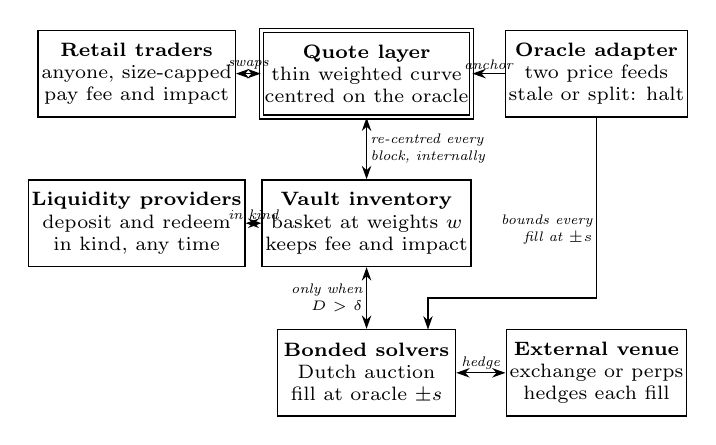
\begin{tikzpicture}[x=1mm,y=1mm,
  box/.style={draw,line width=0.5pt,minimum width=22.6mm,minimum height=11mm,align=center,inner sep=1.2pt,font=\scriptsize,fill=white},
  key/.style={box,double,double distance=0.9pt},
  ttl/.style={font=\scriptsize\bfseries},
  lab/.style={font=\tiny\itshape,inner sep=1.2pt},
  tip/.style={-{Stealth[length=1.7mm,width=1.2mm]},line width=0.45pt},
  both/.style={{Stealth[length=1.7mm,width=1.2mm]}-{Stealth[length=1.7mm,width=1.2mm]},line width=0.45pt}]
\node[box] (ret) at (0,0)   {\textbf{Retail traders}\\anyone, size-capped\\pay fee and impact};
\node[key] (quo) at (29.2,0)  {\textbf{Quote layer}\\thin weighted curve\\centred on the oracle};
\node[box] (ora) at (58.4,0)  {\textbf{Oracle adapter}\\two price feeds\\stale or split: halt};
\node[box] (lps) at (0,-19) {\textbf{Liquidity providers}\\deposit and redeem\\in kind, any time};
\node[box] (vau) at (29.2,-19){\textbf{Vault inventory}\\basket at weights $w$\\keeps fee and impact};
\node[box] (sol) at (29.2,-38){\textbf{Bonded solvers}\\Dutch auction\\fill at oracle $\pm s$};
\node[box] (ext) at (58.4,-38){\textbf{External venue}\\exchange or perps\\hedges each fill};
\draw[both] (ret) -- node[lab,above]{swaps} (quo);
\draw[tip]  (ora) -- node[lab,above]{anchor} (quo);
\draw[both] (lps) -- node[lab,above]{in kind} (vau);
\draw[both] (sol) -- node[lab,above]{hedge} (ext);
\draw[both] (quo) -- node[lab,right,align=left]{re-centred every\\block, internally} (vau);
\draw[both] (vau) -- node[lab,left,align=right]{only when\\$D>\delta$} (sol);
\draw[tip] (ora.south) -- (58.4,-28.5) node[lab,left,align=right,pos=0.62]{bounds every\\fill at $\pm s$} -- (37,-28.5) -- (37,-32.5);
\end{tikzpicture}

\caption{One gated pool. Quotes follow the oracle every block through internal re-centring; inventory moves only when drift exceeds the band $\delta$, through bonded solvers at oracle price $\pm s$.}
\label{fig:arch}
\end{figure}

\subsection{Vault, NAV and drift}
A vault holds $x_i$ of each token. It values itself at oracle prices $p_i$ and measures its drift from target:
\begin{equation}
\NAV=\sum_i x_i p_i,\qquad \omega_i=\frac{x_i p_i}{\NAV},\qquad D=\tfrac12\sum_i\lvert\omega_i-w_i\rvert .
\label{eq:drift}
\end{equation}
$D$ is the one-way notional, as a share of NAV, that restores target weights. LPs mint and redeem in kind: depositing a fraction $\alpha$ of every balance mints $\alpha$ of the share supply, and burning shares returns the same fraction of every balance. Neither path needs a price, so neither can be gamed through the oracle or paused.

\subsection{The gate}
\label{sec:gate}
\paragraph{Trigger.} Every interaction recomputes $D$, and anyone may call a public check. When $D>\delta$ the vault opens a rebalancing intent listing the token deltas that move drift to $\din$.

\paragraph{Reverse Dutch auction.} The spread a solver may keep starts at zero and rises with time, $s(t)=\min(s_{\max},\,\varrho\, t)$, with $\varrho$ = 1\bps\ per second. The first whitelisted solver whose cost is covered fills. With several solvers the fill lands near the cheapest solver's cost plus one step; with one solver it lands at $s_{\max}$, which Section~\ref{sec:costs} treats as the stress case. A solver's cost is the hedge, the same $c$ an arbitrageur pays on a public pool, plus inventory risk on a larger fill.

\paragraph{On-chain invariants.} Every fill must pass four checks, whoever submits it (Table~\ref{tab:inv}). Together they bound the damage of a compromised or hostile solver to $s_{\max}Q_{\max}=0.3\%\times20\%=0.06\%$ of NAV a day, plus any oracle error (Appendix~\ref{app:ex}, B13).


\paragraph{Bonds and fallback.} Solvers post USDC bonds sized to seven days of worst-case damage, so a \$100k bond allows $B/(7s_{\max})\approx\$4.76$M of fills a day. Bonds are slashed only on objective on-chain evidence. If no whitelisted solver fills within $T_{\mathrm{fb}}$ (one hour), the same auction opens to anyone who posts a bond, so the pool stays live without trusting any operator, and a colluding whitelist cannot charge more than outsiders would.

\subsection{The quote layer}
\label{sec:quote}
Closing the inventory to arbitrage would also close it to retail. The quote layer reopens it without reopening arbitrage.

\paragraph{Anchored curve.} At the start of each block the layer sets virtual reserves $\hat x_i=w_i\NAV/p_i$ centred on the oracle. A retail trade executes on these reserves with weighted-pool math and fee $f_q$, and the vault's real balances change by the same amounts; trades in one block move along the curve, and the next block starts again from the oracle. Re-centring is an internal transfer, so the quote stays fresh without the inventory trading. In a public pool the next arbitrageur reverses a retail trade's price impact and keeps it; here the impact stays with LPs, and the inventory change it causes is netted by later flow or rebalanced at the band. A small purchase of token $i$ with token $n$ moves the quote by
\begin{equation}
\Delta\ln P_i\approx\frac{A}{\NAV}\Big(\frac{1}{w_n}+\frac{1}{w_i}\Big),
\label{eq:impact}
\end{equation}
so \$10k of HYPE (10\% weight) paid in USDC (15\%) in a \$10M vault moves it 1.67\% and pays \$30 of fee and \$82 of impact (B10). Because re-centring would let a large trader split an order across blocks, the anchor carries an \emph{inventory skew}: the centre for token $i$ is shifted against the side the vault is already short of, in proportion to $(w_i-\omega_i)/w_i$.

\paragraph{What the quote layer cannot do.} It quotes at a price someone else measured, so it is exposed to anyone who knows the price better or sooner. Section~\ref{sec:oracle} quantifies this. The layer therefore enforces a freshness gate (no trades while the price is older than $\tau_{\max}$ or the feeds disagree), monotone oracle timestamps, a per-window size cap (default 0.1\% of TVL per 12 seconds), and a fee floor tied to realised volatility. The strongest option is \emph{next-price execution}: a trade is submitted in one block and filled at the first oracle price stamped after it, which removes latency and selection edges at the cost of a one-block delay.

\section{Validation}
\label{sec:valid}

The propositions rest on first-order approximations, and Eq.~\eqref{eq:pubn} on a heuristic. We test them against a block-by-block simulation with exact weighted-pool arithmetic, competitive arbitrage to the edge of profitability and LP value measured at true prices (Appendix~\ref{app:sim}). Every design in a scenario runs on the same price paths.

\begin{figure*}[t]
\centering
% Figure 2: loss of a public weighted pool by fee and arbitrage cost (black and white, pgfplots)
\begin{tikzpicture}
\begin{groupplot}[group style={group size=2 by 1,horizontal sep=11mm},
  width=88mm,height=60mm,xmode=log,ymode=log,xmin=1,xmax=100,ymin=0.02,ymax=12,
  xtick={1,2,5,10,20,50,100},xticklabels={1,2,5,10,20,50,100},
  ytick={0.05,0.1,0.2,0.5,1,2,5,10},yticklabels={0.05,0.1,0.2,0.5,1,2,5,10},
  tick style={black,line width=0.4pt},minor tick num=0,tick align=inside,
  every axis/.append style={font=\footnotesize,line width=0.5pt},
  ticklabel style={font=\scriptsize},
  xlabel={Swap fee $f$ (bps)},
  title style={font=\footnotesize,yshift=-1mm},
  legend style={font=\scriptsize,draw=black,line width=0.4pt,fill=white,inner sep=1.5pt,row sep=-1pt,legend cell align=left,at={(0.025,0.025)},anchor=south west},
  legend columns=2,
  cycle list={
   {black,solid,mark=o,mark options={solid,fill=white}},
   {black,dashed,mark=square,mark options={solid,fill=white}},
   {black,dashdotted,mark=triangle,mark options={solid,fill=white}},
   {black,densely dotted,mark=diamond,mark options={solid,fill=white}}}]
\nextgroupplot[title={ETH/USDC 50/50 ($\gamma^{*}=5.28\%$)},ylabel={Loss against benchmark (\% of TVL a year)}]
\addplot[black,line width=0.7pt,solid,forget plot] table[x=f,y=c0]{fig/law_eth.dat};
\addplot[black,only marks,mark=o,mark size=1.9pt,mark options={fill=white,line width=0.5pt},forget plot] table[x=f,y=L]{fig/sim_eth_c0.dat};
\addplot[black,line width=0.7pt,dashed,forget plot] table[x=f,y=c2]{fig/law_eth.dat};
\addplot[black,only marks,mark=square,mark size=1.9pt,mark options={fill=white,line width=0.5pt},forget plot] table[x=f,y=L]{fig/sim_eth_c2.dat};
\addplot[black,line width=0.7pt,dashdotted,forget plot] table[x=f,y=c10]{fig/law_eth.dat};
\addplot[black,only marks,mark=triangle,mark size=1.9pt,mark options={fill=white,line width=0.5pt},forget plot] table[x=f,y=L]{fig/sim_eth_c10.dat};
\addplot[black,line width=0.7pt,densely dotted,forget plot] table[x=f,y=c20]{fig/law_eth.dat};
\addplot[black,only marks,mark=diamond,mark size=1.9pt,mark options={fill=white,line width=0.5pt},forget plot] table[x=f,y=L]{fig/sim_eth_c20.dat};
\addplot[black,line width=0.4pt,domain=1:100,forget plot] {5.28};
\node[font=\scriptsize\itshape,anchor=north east,inner sep=1pt] at (axis cs:95,5.0) {zero-fee loss $\gamma^{*}$};
\addplot[black,line width=0.8pt,domain=1:100,forget plot] {0.1056};
\node[font=\scriptsize\itshape,anchor=north east,inner sep=1pt] at (axis cs:95,0.1) {gated, $s=10$\,bps};
\addplot[black,line width=0.5pt,loosely dashed,domain=1:100,forget plot] {0.3169};
\node[font=\scriptsize\itshape,anchor=south west,inner sep=1pt] at (axis cs:1.1,0.33) {gated, $s=30$\,bps (cap)};
\nextgroupplot[title={Core basket ($\gamma^{*}=8.48\%$)}]
\addplot[black,line width=0.7pt,solid,forget plot] table[x=f,y=c0]{fig/law_core.dat};
\addplot[black,only marks,mark=o,mark size=1.9pt,mark options={fill=white,line width=0.5pt},forget plot] table[x=f,y=L]{fig/sim_core_c0.dat};
\addplot[black,line width=0.7pt,dashed,forget plot] table[x=f,y=c2]{fig/law_core.dat};
\addplot[black,only marks,mark=square,mark size=1.9pt,mark options={fill=white,line width=0.5pt},forget plot] table[x=f,y=L]{fig/sim_core_c2.dat};
\addplot[black,line width=0.7pt,dashdotted,forget plot] table[x=f,y=c10]{fig/law_core.dat};
\addplot[black,only marks,mark=triangle,mark size=1.9pt,mark options={fill=white,line width=0.5pt},forget plot] table[x=f,y=L]{fig/sim_core_c10.dat};
\addplot[black,line width=0.7pt,densely dotted,forget plot] table[x=f,y=c20]{fig/law_core.dat};
\addplot[black,only marks,mark=diamond,mark size=1.9pt,mark options={fill=white,line width=0.5pt},forget plot] table[x=f,y=L]{fig/sim_core_c20.dat};
\addplot[black,line width=0.4pt,domain=1:100,forget plot] {8.48};
\node[font=\scriptsize\itshape,anchor=north east,inner sep=1pt] at (axis cs:95,8.0) {zero-fee loss $\gamma^{*}$};
\addplot[black,line width=0.8pt,domain=1:100,forget plot] {0.104};
\node[font=\scriptsize\itshape,anchor=south east,inner sep=1pt] at (axis cs:95,0.108) {gated, $s=10$\,bps};
\addplot[black,line width=0.5pt,loosely dashed,domain=1:100,forget plot] {0.312};
\node[font=\scriptsize\itshape,anchor=south west,inner sep=1pt] at (axis cs:1.1,0.325) {gated, $s=30$\,bps (cap)};
\addlegendimage{black,line width=0.7pt,solid,mark=o,mark options={solid,fill=white}}\addlegendentry{$c=0$\,bps}
\addlegendimage{black,line width=0.7pt,dashed,mark=square,mark options={solid,fill=white}}\addlegendentry{$c=2$\,bps}
\addlegendimage{black,line width=0.7pt,dashdotted,mark=triangle,mark options={solid,fill=white}}\addlegendentry{$c=10$\,bps}
\addlegendimage{black,line width=0.7pt,densely dotted,mark=diamond,mark options={solid,fill=white}}\addlegendentry{$c=20$\,bps}
\end{groupplot}
\end{tikzpicture}

\caption{Loss of a public weighted pool against the frictionless benchmark, by swap fee and arbitrage cost $c$, with 12-second blocks. Curves: Eq.~\eqref{eq:pub} (ETH/USDC) and Eq.~\eqref{eq:pubn} (core basket). Open markers: simulation, 60--100 one-year paths each; standard errors are smaller than the markers. Horizontal lines: zero-fee loss $\gamma^{*}$, and the gated pool at $\delta=2.5\%$ with a 10\bps\ spread (heavy) and at the 30\bps\ cap (dashed).}
\label{fig:law}
\end{figure*}

\paragraph{Public pools.} Figure~\ref{fig:law} and Table~\ref{tab:valid} compare simulated loss and turnover with the theory. For ETH/USDC, across all 32 combinations tested (fees of 1, 5, 30 and 100\bps; $c$ of 0, 2, 10 and 20\bps\ at 12\,s; $c$ of 0 and 10\bps\ at 2\,s and 0.4\,s), Eq.~\eqref{eq:pub} is within 1.4\% of the simulated loss and 1.2\% of the simulated turnover. For the core basket, Eq.~\eqref{eq:pubn} is within 3\% of the simulated loss whenever $f\ge30$\bps, $c\ge10$\bps\ or blocks are fast. It fails when the overshoot is large relative to the band: at $f=5$\bps, $c=0$ and 12-second blocks it overstates the loss by 15\% (3.02\% against 2.64\%) and understates turnover by 7\%, because one token's arbitrage moves the USDC reserve and with it every other token's mispricing. The public pool then loses less than the formula says, but still 25 times what the gated pool does.

\begin{table}[t]
\centering\footnotesize\setlength{\tabcolsep}{3.3pt}
\caption{Public pools: simulated (sim.) against predicted (th.) turnover ($\times$ TVL a year) and loss (\% of TVL a year). $\Delta t$ in seconds; $f$ and $c$ in bps.}
\label{tab:valid}
\begin{tabular}{lrrrrrrr}
\toprule
Basket & $\Delta t$ & $f$ & $c$ & $T$ sim. & $T$ th. & $L$ sim. & $L$ th.\\
\midrule
\csname @@input\endcsname tab_valid.tex 
\bottomrule
\end{tabular}
\end{table}

\paragraph{Gated vaults.} Table~\ref{tab:gatevalid} checks Proposition~\ref{prop:gate}. Simulated turnover is within 2.3\% of $K/(\delta+\din)$ in all fourteen configurations, for two assets and for the basket, with $K$ computed independently from the drift covariance (A11). The spread is the whole cost: the expected tracking term is a gain of 0.0001--0.06\% a year and grows as $\delta^2$, as A12 predicts. Tracking noise for ETH/USDC matches $\sigma\sqrt{\E[x^2]}$ to within 0.07 points.

\begin{table}[t]
\centering\footnotesize\setlength{\tabcolsep}{2.5pt}
\caption{Gated vaults with $s=10$\bps: turnover against $K/(\delta+\din)$, spread cost, rebalances a year and tracking noise (standard deviation of $\ln V/V_{\mathrm{CRP}}$ after one year; theory in brackets). $\delta$ in \%; 400 (ETH) and 240 (core) paths.}
\label{tab:gatevalid}
\begin{tabular}{lrcrrrrr}
\toprule
& $\delta$ & $\din$ & $T$ sim. & $T$ th. & Cost (\%) & Reb./yr & Noise (\%)\\
\midrule
\csname @@input\endcsname tab_gate.tex 
\bottomrule
\end{tabular}
\end{table}

\paragraph{What the validation does not show.} It shows that the formulas describe the model. Whether the model describes markets is the subject of the next section.

\section{Challenging the assumptions}
\label{sec:challenge}

The baseline makes favourable choices for one side or the other at almost every step. This section relaxes them one at a time. Table~\ref{tab:register} summarises the result; the subsections give the evidence. Unless stated, the core basket is used with $f=30$\bps, $c=s=10$\bps, $\delta=2.5\%$ and 12-second blocks, and every number is a loss in \% of TVL a year.

\begin{table*}[t]
\centering\footnotesize\setlength{\tabcolsep}{3pt}
\caption{Assumption register. ``Public'' is a 30\bps\ public pool, ``gated'' a gated vault at $\delta=2.5\%$; losses in \% of TVL a year for the core basket unless stated.}
\label{tab:register}
\begin{tabular}{L{28mm}L{36mm}L{36mm}L{42mm}L{18mm}}
\toprule
Assumption & Why it may be wrong & Test & Result & Thesis\\
\midrule
Arbitrage costs $c=10$\bps & Top arbitrageurs may pay far less & $c$ from 0 to 20\bps, three block times (Fig.~\ref{fig:be}) & $s^{*}>s_{\max}$ for all $c\ge0.7$\bps; at 12\,s for every $c$ & Holds unless $c<1$\bps\ \emph{and} $\Delta t\le2$\,s\\
Competitive solvers, $s=10$\bps & One solver, or collusion & $s$ at the 30\bps\ cap & Gated 0.31 against public 0.72--2.53 at 12\,s & Holds\\
12-second blocks & Rollups and fast chains & 2\,s and 0.4\,s & Public falls to 2.29 and 2.20; the $c$ term remains & Holds if $c\ge0.7$\bps\\
Volatility level & Crypto volatility varies & All $\sigma$ $\times0.6$ and $\times1.4$ & Public 0.85 and 5.23; gated 0.04 and 0.21 & Holds\\
Constant volatility & Volatility clusters & 2$\times$ regime, 20\% of the time & Public 2.57; gated 0.10 & Holds\\
Zero drift & Trends; mean reversion & Random trends; OU, $\kappa=2$ & Public unchanged; gated $\pm0.2$ & Holds\\
Continuous prices & Jumps & Market and token jumps & Public 4.10; gated 0.12 & Strengthened\\
Oracle equals true price & Lag; pull-oracle price selection & 2--6\,s lag, 6\,s selection, jumps & Quote leak 0.09--0.40; fill selection 1.3 unless timestamps are monotone & Holds with the rules of \S\ref{sec:oracle}\\
Uninformed retail & Toxic flow & Analytic break-even & Positive while informed share $<14\%$ (daily) & Retail only\\
Retail volume $5\times$ & Aggregators route to the cheapest quote & Zero retail & Main result needs none & Holds\\
Basket formula & Cross-token coupling & Simulation & Within 3\% at $f\ge30$\bps; overstates public loss by up to 15\% at 5\bps\ and $c=0$ & Holds; gap smaller at low fees\\
No fixed costs & Gas per fill & 42 fills a year & 0.002--0.02 at \$10M; up to 0.2 at \$1M & Holds above a few \$M\\
\bottomrule
\end{tabular}
\end{table*}

\subsection{Execution costs and solver competition}
\label{sec:costs}

The arbitrageur's cost $c$ is the pivot of the comparison, because it is the only part of the public pool's loss that faster blocks cannot remove and the part the gated pool also pays, as $s$. Figure~\ref{fig:be} plots the break-even spread $s^{*}$ of Proposition~\ref{prop:ratio} against $c$. Against a 30\bps\ public pool, $s^{*}$ exceeds the 30\bps\ cap for every $c\ge0.7$\bps\ at every block time tested, and for every $c$ at 12 seconds ($s^{*}=69$\bps\ at $c=0$). Against a 5\bps\ public pool, the usual tier for majors, $s^{*}$ is at least 73\bps\ everywhere, using the simulated loss where the formula is least accurate. The gated pool can therefore lose on rebalancing cost only if arbitrage is nearly free ($c<1$\bps) on blocks of 2 seconds or less \emph{and} its solvers charge more than 14--30\bps.

\begin{figure}[t]
\centering
% Figure 3: break-even solver spread (black and white, pgfplots)
\begin{tikzpicture}
\begin{axis}[width=\linewidth,height=58mm,ymode=log,xmin=0,xmax=20,ymin=5,ymax=5000,
  xtick={0,5,10,15,20},ytick={5,10,20,50,100,200,500,1000},yticklabels={5,10,20,50,100,200,500,1000},
  tick style={black,line width=0.4pt},minor tick num=0,tick align=inside,
  every axis/.append style={font=\footnotesize,line width=0.5pt},ticklabel style={font=\scriptsize},
  xlabel={Arbitrageur's execution cost $c$ (bps)},ylabel={Break-even solver spread $s^{*}$ (bps)},
  legend style={font=\scriptsize,draw=black,line width=0.4pt,fill=white,inner sep=1.5pt,row sep=-1pt,legend cell align=left,at={(0.025,0.975)},anchor=north west}]
\addplot[black,line width=1.0pt,solid] table[x=c,y=f30dt12]{fig/breakeven.dat};\addlegendentry{$\Delta t=12$\,s}
\addplot[black,line width=1.0pt,dashed] table[x=c,y=f30dt2]{fig/breakeven.dat};\addlegendentry{$\Delta t=2$\,s}
\addplot[black,line width=1.0pt,densely dotted] table[x=c,y=f30dt04]{fig/breakeven.dat};\addlegendentry{$\Delta t=0.4$\,s}
\addplot[black,line width=0.5pt,solid,forget plot] table[x=c,y=f5dt12]{fig/breakeven.dat};
\addplot[black,line width=0.5pt,dashed,forget plot] table[x=c,y=f5dt2]{fig/breakeven.dat};
\addplot[black,line width=0.5pt,densely dotted,forget plot] table[x=c,y=f5dt04]{fig/breakeven.dat};
\node[font=\scriptsize\itshape,anchor=south,inner sep=1pt] at (axis cs:14,760) {public fee 5\,bps (thin)};
\node[font=\scriptsize\itshape,anchor=north,inner sep=1pt] at (axis cs:14,185) {public fee 30\,bps (thick)};
\addplot[black,line width=0.5pt,loosely dashed,domain=0:20] {30};
\node[font=\scriptsize\itshape,anchor=south east,inner sep=1pt] at (axis cs:19.6,31) {spread cap $s_{\max}=30$\,bps};
\addplot[black,line width=0.4pt,domain=0:20] {10};
\node[font=\scriptsize\itshape,anchor=north west,inner sep=1pt] at (axis cs:0.4,9.6) {baseline $s=10$\,bps};
\end{axis}
\end{tikzpicture}

\caption{Break-even solver spread for the core basket at $\delta=2.5\%$: at spreads above a curve the public pool is cheaper. Heavy curves: 30\bps\ public pool; light curves: 5\bps; line style gives the block time.}
\label{fig:be}
\end{figure}

We do not measure $c$. For it to fall below 1\bps, an arbitrageur would have to hedge without paying exchange fees or crossing a spread and without paying for gas, which describes makers with rebates or internalised flow rather than the marginal arbitrageur on most tokens. The solver's cost is at least the same hedge, and larger for larger fills: a gated rebalance trades 2.5\% of NAV at once (\$250k in a \$10M vault, \$25M in a \$1B one), so in a large vault $s$ includes market impact on the hedge venue. Trading back only to $\din=\delta/2$ halves the fill and cuts turnover by a third. With a single solver, or a colluding whitelist, the spread settles at the cap: the gated vault then costs 0.31\% against 0.72\% for a frictionless 30\bps\ public pool and 2.53\% at $c=10$\bps. The cap is enforced by the price-bound invariant, so collusion cannot raise it.

\subsection{Block time}
Faster blocks shrink only the rent term, as $\sqrt{\Delta t}$. At $c=10$\bps\ the public pool's loss falls from 2.53\% at 12 seconds to 2.29\% at 2 seconds and 2.20\% at 0.4 seconds; the floor as $\Delta t\to0$ is $\gamma^{*}c/(f+c)=2.12\%$ (Table~\ref{tab:theory}). Fast chains help public pools a great deal only where arbitrage is also nearly free.

\subsection{Volatility level and regimes}
Both laws scale with variance: $\gamma^{*}$ and $K$ are proportional to $\sigma^2$, while $\rho$ grows only with $\sigma$. Scaling every volatility by 0.6 and by 1.4 gives public losses of 0.854\% and 5.23\% (theory 0.854\% and 5.25\%) and gated losses of 0.038\% and 0.21\% (theory 0.037\% and 0.20\%): a ratio of 22--26 throughout. A two-state regime model, with volatility doubling for 20\% of the time and average variance unchanged, gives 2.57\% $\pm$ 0.05 for the public pool (theory 2.60\%, slightly above baseline because the rent grows with $\sigma^3$) and 0.10\% for the gated vault.

\subsection{Drift: trends and mean reversion}
\label{sec:drift}
With zero drift the benchmark and buy-and-hold have the same expected value. We add random trends (a constant drift per token drawn from $N(0,0.6^2)$ a year) and mean reversion (an Ornstein--Uhlenbeck log price with $\kappa=2$ a year). The public pool's loss does not move (2.52\% and 2.53\%), because its band is too narrow for drift to matter. The gated vault lags its target inside the band, which makes it partly a buy-and-hold portfolio: under trends that earns 0.21\% a year against the benchmark, under mean reversion it costs 0.18\% (0.47\% and 0.37\% at $\din=\delta/2$), against an unchanged spread cost of 0.10\%. These are an order of magnitude smaller than the gap between designs. What does move is the benchmark itself: buy-and-hold beats it by 14.1\% a year under the trend model and trails it by 6.4\% under mean reversion. Holding a constant-weight basket is a bet on mean reversion; this paper only asks what the bet costs to place.

\subsection{Jumps}
With market-wide jumps (26 a year, 4\% standard deviation scaled by each token's volatility) and token-specific jumps (12 a year, 6\%), the public pool's loss rises from 2.53\% to 4.10\%. Jumps add their own excess growth, 1.83\% for this jump model, and a jump overshoots any fee band, so the public pool pays almost all of it. The gated vault's loss rises from 0.10\% to 0.12\%, because jumps add to the variance of drift and the vault pays only the spread on the extra turnover ($1.27\times$ TVL instead of $1.03\times$). Jumps strengthen the thesis, provided the oracle reflects them before anyone trades against the vault, which the next subsection examines.

\subsection{Oracle latency and price selection}
\label{sec:oracle}
The baseline gives the gated pool a perfect oracle. We now let an informed trader see the true price while the quote layer is centred on an oracle that lags by one 2-second block, or three, and let him choose, as a pull oracle allows, the most favourable signed price from a window of three earlier blocks. He trades each token toward the true price up to a pool-wide budget of $q$ of TVL per 12 seconds (C4). Retail flow is $5\times$ TVL a year, the quote fee 30\bps\ and blocks 2 seconds; 40 paths of 60 days per scenario.

\begin{table}[t]
\centering\footnotesize\setlength{\tabcolsep}{3pt}
\caption{Oracle stress on the gated pool with the quote layer, with jumps: informed-trader leak and cost of rebalancing fills (spread plus any price wedge), \% of TVL a year. Without jumps every quote leak is below 0.001\% at a 30\bps\ fee. 2-second blocks, $5\times$ retail; 40 paths of 60 days. $^{\dagger}$Equal to the perfect oracle by construction.}
\label{tab:oracle}
\begin{tabular}{L{40mm}rr}
\toprule
Scenario & Leak & Fill loss\\
\midrule
Perfect oracle & 0 & 0.13\\
Lag 2\,s, cap 0.1\%/12\,s & 0.26 & 0.13\\
Lag 6\,s, cap 0.1\% & 0.35 & 0.13\\
Lag 2\,s, 6\,s selection, cap 0.1\% & 0.40 & 0.13\\
Lag 2\,s, 6\,s selection, cap 0.02\% & 0.09 & 0.13\\
Selection also on rebalancing fills & 0.43 & 1.27\\
Quote fee 10\bps, lag 2\,s, cap 0.1\% & 0.33 & 0.13\\
Quote fee 10\bps, 6\,s selection, cap 0.1\% & 0.71 & 0.12\\
Next-price execution$^{\dagger}$ & 0 & 0.13\\
\bottomrule
\end{tabular}
\end{table}

Three results stand out (Table~\ref{tab:oracle}). First, Gaussian latency is harmless at a 30\bps\ fee: with smooth prices no scenario leaks more than 0.001\% a year, as A16 predicts ($f/\sigma_L=15$ at a 2-second lag). Second, \emph{jumps} are what an informed trader harvests: each jump that lands before the oracle is worth up to the per-window cap, so the leak is 0.26--0.40\% at a cap of 0.1\% and scales with the cap (0.09\% at 0.02\%). Third, and most important, price selection on \emph{rebalancing fills} is the largest oracle risk in the design. If a solver could pick, for each leg, any signed price from the last six seconds, a jump that pushes drift over the band would let him fill at the pre-jump price, and the vault's loss would rise from 0.12\% to 1.3\% $\pm$ 0.2 a year, still far below the public pool's 4.1\% with jumps but ten times the baseline. Without jumps the same selection adds only 0.05\%.

The design therefore requires, and Table~\ref{tab:inv} now enforces: one price set per fill, used both for the trigger and for the price bound; timestamps no older than the newest the vault has already used; and $\tau_{\max}=2$ seconds. With monotone timestamps, the pre-jump price cannot be used once the post-jump price has been, and a fill needs the post-jump price to show drift above the band, so the residual exposure is a jump that lands while an auction is already open. On the quote layer, \emph{next-price execution} removes latency and selection edges entirely; without it the per-window cap bounds the leak, and the cap should be set from the jump rate of each token.

\subsection{Informed retail flow}
Retail pays the fee plus impact, $f+\bar\imath\approx47$\bps\ a dollar at $5\times$ volume. Traders who know the price change $r_H$ over a horizon $H$ trade only when it beats that. The quote layer's retail income stays positive while the informed share of volume is below $\varphi^{*}=(f+\bar\imath)/m$, where $m$ is the average absolute price change on the trades the informed actually make (A17): 49\% for information one hour ahead and 14\% for a day ahead on a 75\%-volatility token (B12). A public pool faces the same arithmetic with a smaller numerator, because it loses most of the impact to arbitrageurs, so informed flow is not a reason to prefer it. It is a reason to treat retail income as uncertain.

\subsection{Retail volume and routing}
Aggregators route each trade to the cheapest venue, so a basket pool with a 30\bps\ quote will win little flow in tokens that trade at 1--5\bps\ elsewhere. The main result needs no retail at all. Retail matters in two ways only: it adds income where it comes (Section~\ref{sec:retail}), and it is the reason a public pool cannot simply raise its fee. A gated pool can set its quote fee for flow rather than for protection, down to the floor set by oracle quality: at 10\bps\ the leak rises to 0.33\% a year with a 2-second lag and 0.71\% with selection (Table~\ref{tab:oracle}), which next-price execution would remove.

\subsection{Fixed costs, pool size and the arbitrage model}
A gated vault makes about 42 fills a year. At \$5--50 of gas per fill that is \$200--2{,}000 a year: 0.002--0.02\% of a \$10M vault but 0.02--0.2\% of a \$1M one, up to twice the spread cost, so the design suits vaults above a few million dollars, or chains with cheap gas. Public arbitrageurs pay gas per trade too, which raises their effective $c$ in small pools. Our arbitrage model assumes perfect competition at the margin; less competition means arbitrageurs wait for larger mispricings, which acts as a larger $c$ in Eq.~\eqref{eq:pub} and raises the public pool's loss. We model arbitrage token by token against USDC; multi-token arbitrage could shave the public pool's turnover somewhat, which is one reason the basket formula is labelled a heuristic.

\section{Retail flow and alternative designs}
\label{sec:retail}

The comparison so far needs no retail flow. Where retail does come, it pays the fee plus price impact, and designs differ in how much of that LPs keep. Table~\ref{tab:retail} gives the net LP result, retail income minus loss against the benchmark, for uninformed retail at 0, 5 and 20 times TVL a year (C5), with 12-second blocks and $c=s=10$\bps.

\begin{table}[t]
\centering\footnotesize\setlength{\tabcolsep}{3pt}
\caption{Net LP result with retail flow, \% of TVL a year: retail income minus loss against the benchmark, by retail volume ($\times$ TVL a year), and at $5\times$ with jumps. Core basket, 12-second blocks, $c=s=10$\bps, 100 paths; standard errors at most 0.04. Single-arbitrageur rows from the earlier simulator (C8).}
\label{tab:retail}
\begin{tabular}{L{37mm}rrrr}
\toprule
Design & $0\times$ & $5\times$ & $20\times$ & Jumps\\
\midrule
\csname @@input\endcsname tab_retail.tex 
\bottomrule
\end{tabular}
\end{table}

\paragraph{Where the income goes.} At $5\times$ volume retail pays 1.50\% of TVL in fees and 0.84\% in impact. A public pool keeps the fee but its arbitrageurs reverse each trade's price impact and keep most of it, paying $c$ on the way; the anchored quote keeps both, because re-centring is internal. The gated pool's lead therefore grows with volume, from 2.4 points over the 30\bps\ public pool with no retail to 2.8 at $5\times$ and 4.0 at $20\times$; with jumps it is 4.4 at $5\times$.

\paragraph{Why the quote is anchored, not synced.} The obvious alternative is a public weighted pool in which one exclusive wallet does all the arbitrage and remits its profit to LPs. It recovers the rent, but in a weighted pool the quote is the inventory, so every sync is a hedged trade. The single-arbitrageur pool is therefore another band rebalancer, with its band set by how fresh it wants its quote to be: syncing whenever the gap reaches $g$ turns over about $\sigma^2/4g$ for two assets, and costs $c\sigma^2/4g$. A fresh quote ($g=0.3\%$) costs the basket 5.1\% a year; a lazy one ($g=1\%$) 1.6\%, with quotes stale enough for informed traders to pick off. The coupling the gate removes is between the price a pool quotes and the inventory it holds; the anchored quote layer moves the price without moving the inventory.

\paragraph{A constant-product version.} A constant-product pool is the two-token, 50/50 case of a weighted pool, so the theory applies with $N=2$, and the gate works for it as for the vault (Table~\ref{tab:cp}). What changes is how a basket is built from pairs. In a hub of token/USDC pairs every pair is half stablecoin, so the basket is 50\% USDC. In a tree of token/token pairs a retail trade crosses several pools and pays several fees. Either way each pair rebalances only inside itself and the pairs' relative sizes drift with the square root of relative prices (A18, B14). On the hub basket, where all designs can hold the same weights, gating cuts the pairs' loss without retail from 1.79\% to 0.16\%, while the 5\bps\ tier common for majors loses 4.3\% without it. Gated pairs appear to beat the gated vault at $5\times$ volume ($+2.47\%$ against $+2.09\%$), only because each pair holds just its token's share of value, so the same trade moves its price further and retail pays 57\bps\ a trade instead of 46: in a gated design that is a pricing choice the vault could match with a higher fee. Pairs drift twice as far from target (2.6\% against 1.2\%), and a cross-pair rebalancer that fixes this turns them into a gated vault split across contracts. The vault therefore stays the base design, and a single token against USDC is a gated pool with $N=2$.

\begin{table}[t]
\centering\footnotesize\setlength{\tabcolsep}{2.4pt}
\caption{Constant-product pairs against weighted designs on the hub basket (50\% USDC): net LP result, \% of TVL a year; retail cost per trade (bps) and average drift from target. 100 paths; standard errors 0.05--0.15.}
\label{tab:cp}
\begin{tabular}{L{25mm}rrrrrr}
\toprule
Design & $0\times$ & $5\times$ & $20\times$ & Jumps & Retail & Drift\\
\midrule
Public weighted, 30\bps & $-2.35$ & $-0.45$ & $+5.22$ & $-1.87$ & 46 & 0.1\%\\
Public CP pairs, 30\bps & $-1.79$ & $+0.09$ & $+6.26$ & $-1.09$ & 57 & 2.3\%\\
Public CP pairs, 5\bps & $-4.29$ & $-4.01$ & $-2.76$ & $-5.28$ & 33 & 2.3\%\\
\addlinespace
Gated weighted vault & $-0.13$ & $+2.09$ & $+9.12$ & $+2.15$ & 46 & 1.2\%\\
Gated CP pairs & $-0.16$ & $+2.47$ & $+11.16$ & $+2.42$ & 57 & 2.6\%\\
Gated CP pairs, cross-pair rebalancing & $-0.21$ & $+2.58$ & $+11.08$ & $+2.69$ & 57 & 1.2\%\\
\bottomrule
\end{tabular}
\end{table}

\section{Related work}
\label{sec:related}
Loss-versus-rebalancing was defined by Milionis et al.\ \cite{lvr}, who also derived arbitrage profits with fees under Poisson block times \cite{lvrfees}; Nezlobin and Tassy \cite{nt} derived LVR under fixed block times with the ladder-height constant of Siegmund \cite{siegmund} and Broadie, Glasserman and Kou \cite{bgk}. Proposition~\ref{prop:pub} adds the arbitrageur's execution cost, which turns out to dominate, and derives the result from a stationarity identity that also gives turnover. Evans \cite{evans} characterised LP returns in geometric-mean markets, and the excess growth rate is Fernholz's \cite{fernholz}. Band rebalancing under proportional costs goes back to Magill and Constantinides \cite{magill} and Davis and Norman \cite{davisnorman}. Among designs, CoW AMM \cite{cowamm} already routes rebalancing to competing solvers through batch auctions; a gated pool adds a chosen drift band for multi-token baskets, fills bounded on-chain at oracle price $\pm s$ and an oracle-anchored retail quote. The auction-managed AMM \cite{amamm} sells the right to the arbitrage flow; Angstrom \cite{angstrom} recaptures it through an off-chain network; QuantAMM \cite{quantamm} moves weights over time but still rebalances through arbitrageurs.

\section{Limitations}
\label{sec:limits}
\begin{itemize}
\item \textbf{No market data.} Volatilities, correlations, jump rates and costs are stylised. Every result is a statement about the model; the formulas make it easy to re-evaluate with measured inputs.
\item \textbf{Arbitrage cost $c$ is the pivot.} The thesis is strongest when $c$ is a few basis points or more and weakest when arbitrage is frictionless on sub-second blocks. $c$ should be measured per token from realised arbitrage trades, including gas and hedge slippage.
\item \textbf{Solver spreads are assumed, not observed.} The bound $s\le s_{\max}$ is enforced on-chain, but where in that range competition settles must be measured with real solvers on realistic fills.
\item \textbf{The basket formula is a heuristic} that overstates public-pool losses by up to 15\% at very low fees and costs.
\item \textbf{Oracle behaviour in fast markets} (staleness, disagreement, jumps between updates) sets the quote layer's leak and must be measured per feed.
\item \textbf{Retail volume and informed share are unknown} for a new venue; the main result does not depend on them, but the retail results of Section~\ref{sec:retail} do.
\item \textbf{Not modelled:} gas as a fixed cost per fill, smart-contract risk, governance, legal form, and strategic behaviour by solvers beyond the spread they charge.
\end{itemize}

\section{Conclusion}
\label{sec:concl}
A weighted pool rebalances whenever its price leaves a band of width fee plus arbitrage cost, and pays that cost plus a block-time overshoot on every dollar: $\Lpub=\gamma^{*}(c+\rho)/(f+c+\rho)$. The formula matches simulation to within 1.4\% for two assets and 3\% for a basket at fees of 30\bps\ or more, and it explains why fees alone cannot protect an index pool: the only lever is a fee high enough to drive away the retail flow that pays LPs. A gated pool removes the coupling. It rebalances at a drift band it chooses, through bonded solvers whose fills are bounded on-chain, and serves retail from a quote anchored to an oracle. For the core basket this cuts the cost of holding target weights from 2.53\% to 0.10\% of TVL a year at 12-second blocks and 10\bps\ costs, and the advantage survives every stress we applied except nearly free arbitrage on blocks of 2 seconds or less combined with solvers that charge more than 14--30\bps. What remains is empirical: measure $c$, solver spreads and oracle behaviour, and the formulas give the answer.

\section*{Disclaimer}
This paper is a draft for discussion. It describes a design that has not been built or audited, and every parameter is a proposal. Results come from models and simulations under stated assumptions; they are not forecasts. Nothing here is financial, investment, legal or tax advice, or an offer to buy any asset.

\section*{Declaration of AI assistance}
This paper was prepared with substantial assistance from a large language model, Claude by Anthropic \cite{claude}, used through the Claude application (Cowork mode) in October 2026; the model identifiers reported by the application were \texttt{claude-opus-5-5} and \texttt{claude-fable-5-1}. The author conceived the research questions and the design, set the scope of each analysis, and reviewed and edited every section. The model derived the formulas of Appendix~\ref{app:deriv}, wrote and ran the simulation code of Appendix~\ref{app:sim}, drafted the text, produced the figures and typeset the document. The author checked the claims, numbers and references and takes full responsibility for the content.

\appendix
\section{Derivations}
\label{app:deriv}

Notation follows Table~\ref{tab:notation}. Token $n$ is USDC with $p_n\equiv1$ and $\Sigma_{nj}=0$. Prices satisfy $dp_i/p_i=\mu_i\,dt+\sigma_i\,dW_i$ with $d\langle W_i,W_j\rangle=\rho_{ij}dt$; the baseline has $\mu_i=0$. Approximations are first order in $f$, $c$, $h$ and $\delta$ unless stated.

\paragraph{A1. Growth of a constant-weight portfolio.} A portfolio with weights $\omega$ has $dV/V=\sum_i\omega_i\,dp_i/p_i$, so $(dV/V)^2=\omega^{\top}\Sigma\omega\,dt$. It\^o's lemma for $\ln V$ gives
\begin{equation}
d\ln V=\sum_i\omega_i\frac{dp_i}{p_i}-\tfrac12\,\omega^{\top}\Sigma\omega\,dt .
\end{equation}
For each token, $d\ln p_i=dp_i/p_i-\tfrac12\sigma_i^2dt$, so $dp_i/p_i=d\ln p_i+\tfrac12\sigma_i^2dt$. Substituting with $\omega=w$:
\begin{equation}
d\ln V_{\mathrm{CRP}}=\sum_i w_i\,d\ln p_i+\underbrace{\tfrac12\Big(\sum_i w_i\sigma_i^2-w^{\top}\Sigma w\Big)}_{\gamma^{*}}dt .
\end{equation}
$\gamma^{*}\ge0$ by Jensen's inequality, since $\sum_iw_i\sigma_i^2$ is the weighted mean of the variances and $w^{\top}\Sigma w$ the variance of the weighted mean.

\paragraph{A2. A frictionless weighted pool tracks the geometric index.} The invariant is $\prod_ix_i^{w_i}=k$. With zero fee and continuous arbitrage the pool's marginal prices equal market prices, which for a weighted pool means $x_ip_i=w_iV$ for every $i$. Substituting $x_i=w_iV/p_i$:
\begin{equation}
\begin{aligned}
k&=\prod_i\Big(\frac{w_iV}{p_i}\Big)^{w_i}=V\prod_i\Big(\frac{w_i}{p_i}\Big)^{w_i}\\
\Rightarrow\;\ln V&=\ln k+\sum_iw_i\ln\frac{p_i}{w_i},
\end{aligned}
\end{equation}
since $\sum_iw_i=1$. Hence $d\ln V_{\mathrm{pool}}=\sum_iw_i\,d\ln p_i$, and by A1, $d\ln(V_{\mathrm{pool}}/V_{\mathrm{CRP}})=-\gamma^{*}dt$. This proves Proposition~\ref{prop:gamma}. With driftless prices $\E[V_{\mathrm{CRP}}(t)]=V_0$, while $\ln V_{\mathrm{pool}}$ has drift $-\tfrac12\sum_iw_i\sigma_i^2$ and variance rate $w^{\top}\Sigma w$, so $\E[V_{\mathrm{pool}}(t)]=V_0e^{-\gamma^{*}t}$.

\paragraph{A3. Two assets.} With one risky token at weight $w$ and USDC at $1-w$: $\sum_iw_i\sigma_i^2=w\sigma^2$ and $w^{\top}\Sigma w=w^2\sigma^2$, so $\gamma^{*}=\tfrac12w(1-w)\sigma^2$, and $\sigma^2/8$ at $w=\tfrac12$.

\paragraph{A4. Reserves against price, and the notional density.} Write $P=\frac{x_n/(1-w)}{x_i/w}$ for the pool's marginal price of token $i$ in USDC. From $x_n=Px_i(1-w)/w$ and $x_i^{w}x_n^{1-w}=k$,
\begin{equation}
x_i^{w}\Big(Px_i\tfrac{1-w}{w}\Big)^{1-w}=k\;\Rightarrow\;x_i=k\Big(\frac{w}{(1-w)P}\Big)^{1-w},
\end{equation}
so $d\ln x_i=-(1-w)\,d\ln P$ and $d\ln x_n=w\,d\ln P$. A trade that moves the log price by $dz$ exchanges $p\,|dx_i|=(1-w)\,x_ip\,|dz|=w(1-w)V|dz|$ dollars, using $x_ip=wV$ near the market. We call $\nu=w(1-w)V$ the \emph{notional density}: dollars traded per unit of log-price movement.

\paragraph{A5. The band.} Let $z=\ln P-\ln p$ be the pool's mispricing. The pool's ask, fee included, is $P/(1-f)$ and its bid $P(1-f)$. An arbitrageur can sell token $i$ elsewhere for $p(1-c)$ and buy it for $p(1+c)$. Buying from the pool is profitable when $P/(1-f)<p(1-c)$, that is $z<\ln(1-f)+\ln(1-c)\equiv-h_-$; selling to it when $P(1-f)>p(1+c)$, that is $z>\ln(1+c)-\ln(1-f)\equiv h_+$. The half-width is
\begin{equation}
\begin{aligned}
h&=\tfrac12(h_++h_-)=\tfrac12\ln\frac{1+c}{1-c}-\ln(1-f)\\
&=f+c+\tfrac12f^2+O(f^3,c^3).
\end{aligned}
\end{equation}
Competition makes him trade at the first block where $z$ is outside $[-h_-,h_+]$, and only up to the edge, where his marginal profit is zero.

\paragraph{A6. Loss per trade.} Suppose a block finds $z=-h_--R$ with $R>0$. The arbitrageur buys until $z=-h_-$. When the pool's log price is $u\in[-h_--R,-h_-]$, it sells at log price $u-\ln(1-f)$, which lies $v+c'$ below the market, with $c'=-\ln(1-c)\approx c$ and $v=-h_--u\in[0,R]$. With $\nu$ dollars per unit of $z$ (A4), the LP's loss against the market price is
\begin{equation}
\ell(R)=\nu\int_0^R(c+v)\,dv=\nu\big(cR+\tfrac12R^2\big).
\end{equation}
The arbitrageur pays $c$ on the $\nu R$ dollars he hedges, so his profit is $\nu R^2/2$. The fee never appears: it stays in the pool and only shifts the edge.

\paragraph{A7. The push identity.} Let $Y_k=z_k+h_-\in[0,H]$, $H=2h$, be the position inside the band after block $k$, and $\varepsilon_k=-(\ln p_{k+1}-\ln p_k)$ the market move, with $\E[\varepsilon_k^2]=\sigma^2\Delta t$. With pushes $U_k=(Y_k+\varepsilon_k-H)^+$ at the top and $L_k=(-Y_k-\varepsilon_k)^+$ at the bottom,
\begin{equation}
Y_{k+1}=Y_k+\varepsilon_k-U_k+L_k .
\end{equation}
Squaring case by case: with no trade $Y_{k+1}^2=(Y_k+\varepsilon_k)^2$; with a top trade $Y_{k+1}^2=H^2=(Y_k+\varepsilon_k)^2-2HU_k-U_k^2$; with a bottom trade $Y_{k+1}^2=0=(Y_k+\varepsilon_k)^2-L_k^2$. In every case
\begin{equation}
Y_{k+1}^2=Y_k^2+2Y_k\varepsilon_k+\varepsilon_k^2-2HU_k-U_k^2-L_k^2 .
\end{equation}
In the stationary state $\E[Y_{k+1}^2]=\E[Y_k^2]$ and $\E[Y_{k+1}]=\E[Y_k]$. The market move $\varepsilon_k$ is independent of $Y_k$ with mean $\bar\varepsilon=\tfrac12\sigma^2\Delta t$, and the second condition gives $\E[U_k]-\E[L_k]=\bar\varepsilon$. Writing $2H\E[U_k]=H(\E[U_k]+\E[L_k])+H\bar\varepsilon$, the expectation of the squared recursion is
\begin{equation}
\sigma^2\Delta t+2\E[Y]\bar\varepsilon=H(\E[U]+\E[L])+H\bar\varepsilon+\E[U^2]+\E[L^2].
\end{equation}
The two drift terms cancel when $\E[Y]=H/2$, which holds by symmetry up to corrections of relative order $h$; the remainder is $O(h\sigma^2\Delta t)$ against $\sigma^2\Delta t$. Summing over a year, with $\Pi=\sum(U_k+L_k)$ and $M=\sum(U_k^2+L_k^2)$,
\begin{equation}
\sigma^2=2h\,\Pi+M\quad\Longrightarrow\quad \Pi=\frac{\sigma^2}{2(h+\rho)},\qquad \rho\equiv\frac{M}{2\Pi}.
\end{equation}
Apart from that first-order step, the identity uses no assumption on the distribution of the overshoots.

\paragraph{A8. Turnover and loss.} Each unit of push trades $\nu$ dollars (A4) and costs the LP $c$ per dollar plus the overshoot term of A6. Per year, as a share of TVL,
\begin{align}
\Tpub&=\frac{\nu\Pi}{V}=\frac{w(1-w)\sigma^2}{2(h+\rho)}=\frac{\gamma^{*}}{h+\rho},\\
\Lpub&=\frac{\nu}{V}\big(c\,\Pi+\tfrac12M\big)=w(1-w)\Pi(c+\rho)=\gamma^{*}\frac{c+\rho}{h+\rho},
\end{align}
using $\gamma^{*}=\tfrac12w(1-w)\sigma^2$ (A3). The loss splits into the hedging cost $\gamma^{*}c/(h+\rho)$, paid to external venues, and the arbitrage rent $\gamma^{*}\rho/(h+\rho)$, shared between arbitrageurs and block producers. This proves Proposition~\ref{prop:pub} given $\rho$.

\paragraph{A9. The overshoot constant.} Consider the fast-block regime $\sigma\sqrt{\Delta t}\ll h$. After a top trade the band's top edge sits at the market's current log price. The next top trade happens at the first block where the market exceeds that level, and the push is the excess: top trades are the strict ascending ladder epochs of the random walk $-\ln p$, and the pushes are its ladder heights $H$. The exception is the first top trade after a bottom trade, a first passage over a level about $2h$ away; since a bottom trade needs a $2h$ drawdown, such trades are a fraction $O(\sigma\sqrt{\Delta t}/h)$ of all trades. For a Gaussian random walk with step standard deviation $\sigma\sqrt{\Delta t}$, renewal theory gives \cite{siegmund,bgk,nt}
\begin{equation}
\frac{\E[H^2]}{2\E[H]}=\beta\sigma\sqrt{\Delta t},\qquad \beta=-\frac{\zeta(1/2)}{\sqrt{2\pi}}=0.5826,
\end{equation}
the same constant that shifts a discretely monitored barrier \cite{bgk}. Hence $\rho=\beta\sigma\sqrt{\Delta t}\,[1+O(\sigma\sqrt{\Delta t}/h)]$. At the opposite extreme, $h\to0$, the pool trades every block, pushes are $|\varepsilon_k|$, and $\rho=\E[\varepsilon^2]/2\E|\varepsilon|=\sqrt{\pi/8}\,\sigma\sqrt{\Delta t}=0.627\,\sigma\sqrt{\Delta t}$; Eq.~\eqref{eq:pub} then gives $L=\gamma^{*}$ at $f=c=0$ for any $\rho$. A direct simulation with $7\times10^{6}$ ladder heights of a Gaussian walk gives $\E[H^2]/2\E[H]=0.584$, within 0.3\% of $\beta$.

\paragraph{A10. Baskets.} In a weighted pool of $n-1$ risky tokens and USDC, an arbitrage of token $i$ against USDC changes only $x_i$ and $x_n$; with $x_i^{w_i}x_n^{w_n}$ fixed, the notional density of pair $i$ is $w_iw_n/(w_i+w_n)\,V$ and its trades shift every other token's price through $x_n$. We do not solve this coupled problem. We apply A8 token by token, assigning each token the share $\gamma_i/\sum_j\gamma_j$ of $\gamma^{*}$ with $\gamma_i=\tfrac12w_i(1-w_i)\sigma_i^2$, its two-asset premium against the rest of the pool, and its own $\rho_i=\beta\sigma_i\sqrt{\Delta t}$:
\begin{equation}
\Lpub\approx\gamma^{*}\sum_i\frac{\gamma_i}{\sum_j\gamma_j}\,\frac{c+\rho_i}{h+\rho_i}\approx\gamma^{*}\frac{c+\bar\rho}{h+\bar\rho},
\end{equation}
where the second step linearises in $\rho_i$ around $\bar\rho=\beta\sigma_{\mathrm{eff}}\sqrt{\Delta t}$, $\sigma_{\mathrm{eff}}=\sum_i\gamma_i\sigma_i/\sum_i\gamma_i$. The justification is empirical (Table~\ref{tab:valid}).

\paragraph{A11. Gated turnover.} Between rebalances the weights evolve as $d\omega=(\mathrm{diag}(\omega)-\omega\omega^{\top})\,dp/p$, so near target the drift vector $x=\omega-w$ has covariance rate
\begin{equation}
\Omega=(\mathrm{diag}(w)-ww^{\top})\,\Sigma\,(\mathrm{diag}(w)-ww^{\top})
\end{equation}
and a drift of order $\sigma^2$ (A12), which changes $K$ only at second order in $\delta$. \emph{Two assets:} $x_1=-x_2=x$, $D=|x|$ and $dx=w(1-w)\sigma\,dW$, so $K=w^2(1-w)^2\sigma^2$. The expected exit time $u(x)$ from $(-\delta,\delta)$ solves $\tfrac12Ku''=-1$ with $u(\pm\delta)=0$, so $u(x)=(\delta^2-x^2)/K$ and $\E[\tau]=u(\din)=(\delta^2-\din^2)/K$. Each trip ends with a trade of $\delta-\din$, hence
\begin{equation}
\Tgat=\frac{\delta-\din}{(\delta^2-\din^2)/K}=\frac{K}{\delta+\din}.
\end{equation}
\emph{Baskets:} $D=\tfrac12\|x\|_1$ is not a one-dimensional diffusion, but Brownian scaling ($x\to ax$, $t\to a^2t$) makes $\E[\tau_\delta]$ proportional to $\delta^2$, so $K\equiv\delta^2/\E[\tau_\delta]$ is a constant of the basket. We compute it by simulating the Gaussian process with covariance $\Omega$ from zero until $\tfrac12\|x\|_1=\delta$: $K=0.0260$ for the core basket, the same at $\delta=1\%$ and $2.5\%$ (0.0262 and 0.0260). Neither simple closed form fits: $(\tfrac12\sum_i\sqrt{\Omega_{ii}})^2=0.035$ and $\tfrac12\operatorname{tr}\Omega=0.013$. For $\din>0$ in several dimensions we use $\E[\tau]\approx(\delta^2-\din^2)/K$, checked in Table~\ref{tab:gatevalid}.

\paragraph{A12. Tracking.} Over $dt$, a portfolio with weights $\omega=w+x$ has expected log growth $\omega^{\top}\mu-\tfrac12\omega^{\top}\Sigma\omega$ (A1). Subtracting the benchmark's,
\begin{equation}
\frac{d}{dt}\E\big[\ln V-\ln V_{\mathrm{CRP}}\big]=x^{\top}\mu-w^{\top}\Sigma x-\tfrac12x^{\top}\Sigma x .
\end{equation}
\emph{Two assets, $\din=0$, $\mu=0$.} The vault restarts at $x=0$ after every exit, so the stationary density of $x$ is the occupation density of Brownian motion started at 0 and killed at $\pm\delta$, which is proportional to the Green's function $\delta-|x|$: a triangle. Hence
\begin{equation}
\E[x^2]=\frac{\int_{-\delta}^{\delta}x^2(\delta-|x|)dx}{\int_{-\delta}^{\delta}(\delta-|x|)dx}=\frac{2(\delta^4/3-\delta^4/4)}{\delta^2}=\frac{\delta^2}{6}.
\end{equation}
With driftless prices the risky weight drifts down: from $\omega=a/(a+b)$ with $da=a\sigma dW$, It\^o gives $d\omega=\omega(1-\omega)\sigma dW-\omega^2(1-\omega)\sigma^2dt$. A drift $m=-w^2(1-w)\sigma^2$ shifts the mean by $\E[x]\approx m\delta^2/(6K)=-\delta^2/(6(1-w))$ to first order in $m\delta/K$ (solve $\tfrac12Ku''+mu'=-x$, $u(\pm\delta)=0$, and divide $u(0)$ by $\E[\tau]$). The expected drag is therefore
\begin{equation}
L_{\mathrm{track}}=\tfrac12\sigma^2\E[x^2]+w\sigma^2\E[x]=\sigma^2\delta^2\Big(\frac1{12}-\frac{w}{6(1-w)}\Big),
\end{equation}
which is $-\sigma^2\delta^2/12$ at $w=\tfrac12$: a gain of 0.002\% a year at $\sigma=65\%$, $\delta=2.5\%$ (simulation: 0.000--0.006\%, within sampling error). The tracking \emph{noise}, the standard deviation of $\ln(V/V_{\mathrm{CRP}})$ after one year, is $\sqrt{\E[x^{\top}\Sigma x]}=\sigma\sqrt{\E[x^2]}=\sigma\delta/\sqrt6$.

\paragraph{A13. Ratio and break-even.} Dividing Eq.~\eqref{eq:pub} by Eq.~\eqref{eq:gate} with $L_{\mathrm{track}}$ neglected gives Eq.~\eqref{eq:ratio}. Setting the ratio to one gives $s^{*}$. Setting $\Lpub(f)=\Lgat$ and solving $(c+\rho)/(h+\rho)=r$, with $r=sK/(\gamma^{*}(\delta+\din))$, gives $h^{*}=(c+\rho)/r-\rho$; with $h\approx f+c$ the matching public fee is $f^{*}\approx(c+\rho)(1/r-1)$. At fees of several percent the first-order band is no longer accurate, so Table~\ref{tab:theory} solves Eq.~\eqref{eq:h} for $f$ exactly.

\paragraph{A14. The public pool in weight terms.} A rule that trades back to the edge of a weight band $\pm\delta_{\mathrm{eq}}$ has, by A11 with $\din\to\delta$, turnover $K/2\delta_{\mathrm{eq}}$. Equating to $\Tpub=\gamma^{*}/(h+\rho)$ gives $\delta_{\mathrm{eq}}=K(h+\rho)/2\gamma^{*}$, which is $w(1-w)(h+\rho)$ for two assets.

\paragraph{A15. Price impact on the quote layer.} Buying token $i$ with $dn$ of token $n$ on virtual reserves changes the pair price $P=(x_n/w_n)/(x_i/w_i)$ by $d\ln P=dn/x_n+dx_i/x_i$ with $dx_i\approx dn/P$. With $x_n=w_n\NAV/p_n$ and $Px_i=(w_i/w_n)x_n$,
\begin{equation}
d\ln P=\frac{dn}{\NAV}\Big(\frac1{w_n}+\frac1{w_i}\Big).
\end{equation}
A buy of size $A$ pays on average half the final move, $\tfrac12A^2(1/w_n+1/w_i)/\NAV$, plus the fee.

\paragraph{A16. Latency and selection on the quote layer.} Let the quote be centred on a price that differs from the true price by a log gap $X$. A trader who knows $X$ buys or sells up to the cap $q$ per window when $|X|$ exceeds the fee plus impact. With fee $f$ alone and $X\sim N(0,\sigma_L^2)$, $\sigma_L=\sigma\sqrt{L}$ for an oracle lag $L$, the leak per window is
\begin{equation}
q\,\E\big[(|X|-f)^+\big]=2q\Big[\sigma_L\varphi\Big(\frac{f}{\sigma_L}\Big)-f\Big(1-\Phi\Big(\frac{f}{\sigma_L}\Big)\Big)\Big].
\end{equation}
With a pull oracle and freshness window $\tau$, the trader may choose any signed price from the last $\tau$ seconds. The best one for buying is the minimum of the path over the window, whose distance from the current price is the maximum of a Brownian motion over $\tau$; by the reflection principle it is distributed as $|N(0,\sigma^2\tau)|$ on each side. Selection therefore turns a lag of $L$ into a lag of about $L+\tau$, with the better of two sides. A jump $J$ between the true price and the oracle gives an edge of $|J|-f$ on up to $q$ of TVL, so jumps at rate $\lambda$ leak about $\lambda q\,\E[(|J|-f-\bar\imath)^+]$ a year, where $\bar\imath$ is the average impact paid. Next-price execution sets $X$ to zero by construction.

\paragraph{A17. Informed flow.} Let retail pay the fee $f$ and average impact $\bar\imath$ per dollar, $k=f+\bar\imath$, and let a fraction $\varphi$ of volume come from traders who know the price change $r_H$ over a horizon $H$ and trade only when $|r_H|>k$. Their trades earn $m-k$ a dollar, with $m=\E[\,|r_H|\,\big|\,|r_H|>k]$; for $r_H\sim N(0,s^2)$, $m=s\varphi(k/s)/(1-\Phi(k/s))$. LP income per dollar of volume is $(1-\varphi)k-\varphi(m-k)=k-\varphi m$, positive while $\varphi<\varphi^{*}=k/m$.

\paragraph{A18. Constant-product pairs.} A 50/50 pair of token $i$ and USDC, rebalanced continuously at fair prices, has $d\ln V=\tfrac12d\ln p_i+\tfrac18\sigma_i^2dt$ by A1, so $V(t)=V(0)\sqrt{p_i(t)/p_i(0)}\,e^{\sigma_i^2t/8}$. Pairs on different tokens change relative size with the square root of relative prices, so a basket built from pairs drifts unless value is moved between them.

\section{Worked examples}
\label{app:ex}

Each example recomputes a number used in the text from the formulas of Appendix~\ref{app:deriv}. A year has $3.1536\times10^{7}$ seconds; 1\bps\ $=10^{-4}$.

\paragraph{B1. Excess growth rates.} \emph{ETH/USDC:} $\gamma^{*}=\tfrac12\cdot0.5\cdot0.5\cdot0.65^2=0.125\times0.4225=0.0528$, or 5.28\% a year. \emph{Core basket:} the weighted mean variance is
\[
\begin{aligned}\textstyle\sum_iw_i\sigma_i^2&=0.30(0.25)+0.25(0.4225)+0.15(0.64)\\&\quad+0.10(1.00)+0.05(0.64)=0.4086 .\end{aligned}
\]
The basket variance $w^{\top}\Sigma w$ has a diagonal part $\sum_iw_i^2\sigma_i^2=0.0749$ and a cross part $\sum_{i\ne j}w_iw_j\rho_{ij}\sigma_i\sigma_j=0.1641$ (the BTC--ETH pair alone contributes $2\cdot0.30\cdot0.25\cdot0.80\cdot0.50\cdot0.65=0.0390$), so $w^{\top}\Sigma w=0.2390$ and the basket's volatility is $\sqrt{0.2390}=48.9\%$. Then $\gamma^{*}=\tfrac12(0.4086-0.2390)=0.0848$, or 8.48\%.

\paragraph{B2. Overshoot.} For 12-second blocks $\sqrt{\Delta t}=\sqrt{12/3.1536\times10^{7}}=6.169\times10^{-4}$. For ETH, $\sigma\sqrt{\Delta t}=4.01$\bps\ and $\rho=0.5826\times4.01=2.34$\bps; with 2-second blocks 0.95\bps, with 0.4-second blocks 0.43\bps. For the core basket, $\gamma_i=\tfrac12w_i(1-w_i)\sigma_i^2$ is 0.0263, 0.0396, 0.0408, 0.0450 and 0.0152 for BTC, ETH, SOL, HYPE and LINK (sum 0.1669), so
\[
\begin{aligned}\sigma_{\mathrm{eff}}&=\big[0.0263(0.5)+0.0396(0.65)+0.0408(0.8)\\&\quad+0.0450(1.0)+0.0152(0.8)\big]/0.1669=0.771,\end{aligned}
\]
and $\bar\rho=0.5826\times0.771\times6.169\times10^{-4}=2.77$\bps\ (1.13\bps\ at 2\,s, 0.51\bps\ at 0.4\,s).

\paragraph{B3. Band.} At $f=30$\bps\ and $c=10$\bps: $h_+=\ln(1.001/0.997)=40.04$\bps\ and $h_-=-\ln(0.997\times0.999)=40.05$\bps, so $h=40.05$\bps, against $f+c+f^2/2=40.045$\bps.

\paragraph{B4. Public ETH/USDC pool.} $f=30$, $c=10$\bps, 12\,s: $h+\rho=40.05+2.34=42.38$\bps. Turnover $\Tpub=0.0528/0.004238=12.46\times$ TVL a year. Loss $\Lpub=0.0528\times12.34/42.38=1.537\%$, of which hedging $0.0528\times10/42.38=1.246\%$ and rent $0.291\%$. Simulation: $12.48\times$ and 1.539\%. The weight band is $\delta_{\mathrm{eq}}=0.25\times42.38=10.6$\bps\ of weight.

\paragraph{B5. Public core-basket pool.} Same parameters: $h+\bar\rho=42.82$\bps, $\Tpub=0.0848/0.004282=19.81$, $\Lpub=0.0848\times12.77/42.82=2.530\%$ (hedging 1.981\%, rent 0.549\%). Simulation: 19.81 and 2.526\%. With blocks infinitely fast the loss falls only to $0.0848\times10/40.05=2.12\%$ (ETH/USDC: 1.32\%).

\paragraph{B6. Zero arbitrage cost.} ETH/USDC at 30\bps\ and 12\,s with $c=0$: $h=-\ln0.997=30.05$\bps\ and $\Lpub=0.0528\times2.34/32.39=0.381\%$; simulation 0.381\%. The Poisson-block formula \cite{lvrfees} gives $P_{\mathrm{trade}}=1/(1+f\sqrt{2/\Delta t}/\sigma)=1/(1+0.003\times2293/0.65)=0.0863$ and a loss of $0.0528\times0.0863=0.456\%$. With 0.4-second blocks Eq.~\eqref{eq:pub} gives $0.0528\times0.43/30.48=0.074\%$; simulation 0.074\%.

\paragraph{B7. Gated pool.} ETH/USDC: $K=(0.25\times0.65)^2=0.0264$. At $\delta=2.5\%$, $\din=0$: $\Tgat=0.0264/0.025=1.056$, so a 10\bps\ spread costs 0.106\% a year; the vault rebalances about $1.056/0.025=42$ times a year, each time trading 2.5\% of NAV (\$250k in a \$10M vault). With $\din=\delta/2$: $0.0264/0.0375=0.704$, 0.070\% a year, 56 smaller fills. Core basket: $K=0.0260$, $\Tgat=1.04$, 0.104\% at $s=10$\bps\ and 0.312\% at the cap of 30\bps.

\paragraph{B8. Tracking.} At $\delta=2.5\%$: $\E[x^2]=\delta^2/6=1.04\times10^{-4}$, so tracking noise is $0.65\times\sqrt{1.04\times10^{-4}}=0.66\%$ per $\sqrt{\text{year}}$ (simulation 0.69\%). The expected drag at $w=\tfrac12$ is $-\sigma^2\delta^2/12=-0.4225\times6.25\times10^{-4}/12=-0.002\%$ a year, a gain too small to matter.

\paragraph{B9. Ratio, break-even and matching fee.} Core basket, 12\,s, $c=10$\bps, $f=30$\bps, $\delta=2.5\%$, $s=10$\bps. Turnover ratio $\gamma^{*}\delta/K(h+\bar\rho)=0.0848\times0.025/(0.0260\times0.004282)=19.0$; cost-per-dollar ratio $(c+\bar\rho)/s=12.77/10=1.28$; loss ratio $19.0\times1.28=24.3$. Break-even spread $s^{*}=\Lpub\,\delta/K=0.0253\times0.025/0.026=243$\bps. Matching public fee: $r=sK/\gamma^{*}\delta=0.001\times0.026/(0.0848\times0.025)=0.0123$, so to first order $f^{*}=12.77\times(1/0.0123-1)=1{,}028$\bps; solving Eq.~\eqref{eq:h} exactly for $h^{*}=12.77/0.0123-2.77=1{,}039$\bps\ gives $f^{*}=9.8\%$. With $c=0$ and 0.4-second blocks: $\Lpub=0.0848\times0.51/30.56=0.140\%$, ratio 1.35, $s^{*}=0.0014\times0.025/0.026=13.5$\bps.

\paragraph{B10. Price impact.} \$10k of HYPE ($w_i=0.10$) bought with USDC ($w_n=0.15$) in a \$10M vault: Eq.~\eqref{eq:impact} gives $10^{-3}\times(6.67+10)=1.67\%$. On exact virtual reserves ($\hat x_n=\$1.5$M, $\hat x_i=\$1.0$M of HYPE) with a 30\bps\ fee, the buyer receives \$9{,}888 of HYPE for \$10{,}000: \$30 of fee and \$82 of impact.

\paragraph{B11. Gaussian latency leak.} At $\sigma=80\%$ and a 2-second lag, $\sigma_L=0.8\sqrt{2/3.1536\times10^{7}}=2.0$\bps; a 30\bps\ fee is $15\sigma_L$ and A16 gives a leak of zero to any precision. A 10\bps\ fee with an effective lag of 8 seconds (2\,s lag plus a 6\,s selection window) has $\sigma_L=4.0$\bps, $f/\sigma_L=2.5$ and a leak of $1.7\times10^{-6}$ per dollar per window; at 0.1\% of TVL per 12-second window, $2.63\times10^{6}$ windows a year give 0.45\% of TVL a year. \emph{Jumps:} the jump model has about $26+5\times12=86$ jumps a year; each is worth at most $q$ times the jump net of fee and impact, about 3--4\% on average, so at $q=0.1\%$ the leak is about $86\times0.001\times0.035\approx0.3\%$ a year (simulation 0.26\%).

\paragraph{B12. Informed flow.} With $k=f+\bar\imath=30+17=47$\bps\ (the average fee plus impact paid at $5\times$ volume, Section~\ref{sec:retail}) and a token at 75\% volatility, a trader who knows tomorrow's price faces $s=0.75\sqrt{1/365}=3.93\%$; $k/s=0.12$, so $m=3.44\%$ and $\varphi^{*}=0.47/3.44=14\%$. For next-hour information $s=0.80\%$, $k/s=0.59$, $m=0.97\%$ and $\varphi^{*}=49\%$.

\paragraph{B13. Worst case for a solver.} $s_{\max}Q_{\max}=0.003\times0.20=0.06\%$ of NAV a day. Bond capacity: $\$100{,}000/(7\times0.003)=\$4.76$M of fills a day.

\paragraph{B14. Drift of a basket of pairs.} Two constant-product pairs of equal value, one on a token that doubles and one on a token that stays flat: by A18 their values become $\sqrt2=1.414$ and 1, so the basket holds 58.6\% and 41.4\% instead of 50/50, a drift of 8.6\% that no trade inside either pair can correct.

\paragraph{B15. Volatility scaling.} Scaling every $\sigma_i$ by 1.4 multiplies $\gamma^{*}$ and $K$ by $1.96$ and $\bar\rho$ by 1.4: $\gamma^{*}=0.1662$, $\bar\rho=3.88$\bps, so $\Lpub=0.1662\times13.88/43.93=5.25\%$ and $\Lgat=0.104\%\times1.96=0.204\%$. At 0.6: $\gamma^{*}=0.0305$, $\bar\rho=1.66$\bps, $\Lpub=0.0305\times11.66/41.71=0.854\%$ and $\Lgat=0.104\%\times0.36=0.037\%$.

\paragraph{B16. Volatility regimes.} With average variance fixed, the low state scales volatility by $m_L=1/\sqrt{0.8+0.2\times4}=0.791$ and the high state by $2m_L=1.581$. In the low state $\gamma^{*}=0.0848\times0.625=0.0530$ and $\bar\rho=2.19$\bps, so the loss rate is $0.0530\times12.19/42.24=1.53\%$; in the high state $\gamma^{*}=0.2120$, $\bar\rho=4.38$\bps\ and $0.2120\times14.38/44.43=6.86\%$. Weighting by time, $0.8\times1.53+0.2\times6.86=2.60\%$ (simulation $2.57\pm0.05$). The gated cost is linear in variance, so its average is unchanged at 0.104\%.

\paragraph{B17. Excess growth of jumps.} A market-wide jump moves token $i$ by $\beta_i\times4\%$ times a standard normal, with $\beta_i=\sigma_i/0.65$ (0.77, 1.00, 1.23, 1.54 and 1.23), 26 times a year; each token also jumps by 6\% times a standard normal 12 times a year. The jump covariance a year is therefore $J_{ij}=26(0.04\beta_i)(0.04\beta_j)+12(0.06)^2\mathbf 1_{i=j}$; for ETH $J_{ii}=0.0416+0.0432=0.0848$. Then $\sum_iw_iJ_{ii}=0.0770$, $w^{\top}Jw=0.0404$ and the jumps' own excess growth is $\tfrac12(0.0770-0.0404)=1.83\%$, which the public pool almost entirely pays: its loss rises by 1.57 points.

\paragraph{B18. Gas per fill.} A gated vault rebalancing 42 times a year at \$5 to \$50 of gas per fill spends \$210 to \$2{,}100 a year: 0.002--0.021\% of a \$10M vault and 0.02--0.21\% of a \$1M vault, against a spread cost of 0.104\%.

\section{Simulation methods}
\label{app:sim}

\paragraph{C1. Prices.} A Monte Carlo program in C (\texttt{sim\_v.c}, xoshiro256** generator, Box--Muller normals) advances all prices one block at a time with exact log-normal steps, $\ln p_{i,k+1}-\ln p_{i,k}=-\tfrac12\sigma_i^2\Delta t+\sigma_i\sqrt{\Delta t}\,(Lz_k)_i$, where $L$ is the Cholesky factor of the correlation matrix. Core-basket volatilities are 50, 65, 80, 100 and 80\%; correlations are BTC--ETH 0.80, BTC--SOL 0.70, BTC--HYPE 0.50, BTC--LINK 0.65, ETH--SOL 0.75, ETH--HYPE 0.50, ETH--LINK 0.75, SOL--HYPE 0.50, SOL--LINK 0.65 and HYPE--LINK 0.45. Runs cover one year with 12-second blocks, or 60 days (2\,s) and 12 days (0.4\,s), annualised. All designs in a scenario share the price path and the retail stream.

\paragraph{C2. Public pools.} In every block each risky token is arbitraged against USDC, in two passes over the tokens. The arbitrageur trades on the exact weighted-pool curve, with the fee charged on the input, until the pool's ask equals $p(1-c)$ or its bid equals $p(1+c)$, using the closed form from the pair invariant $x_i^{w_i}x_n^{w_n}$. The LP's loss is the change in pool value at true prices; turnover is the notional at true prices.

\paragraph{C3. Gated vaults.} At the end of each block the vault computes $D$ at true prices. If $D>\delta$ it sets weights to $w+(\din/D)(\omega-w)$ and deducts $s(D-\din)$ of NAV. In the price-selection stress the solver also chooses, for each leg, the least favourable price for the vault among the last $m$ blocks, and the vault loses that wedge on the leg's notional.

\paragraph{C4. Quote layer and informed trader.} Retail trades virtual reserves $\hat x_k=w_k\NAV/p_k$ with weighted-pool math and fee $f_q$; real balances change by the same amounts. The informed trader acts before retail in each block: for each token it trades toward the true price on a curve centred on an oracle price that lags by $\ell$ blocks, or, with selection, on the most favourable price in the $m$ blocks before that, until its marginal profit is zero or a pool-wide budget is spent. The budget refills at $q$ of TVL per 12 seconds and holds at most $q$.

\paragraph{C5. Retail flow.} Trades arrive as a Poisson process with intensity (volume/TVL)/(mean size) a year; sizes are lognormal with mean 0.01\% of TVL and log standard deviation 1; the token is drawn in proportion to weight and the side with equal odds. Retail is uninformed.

\paragraph{C6. Stress scenarios.} \emph{Volatility}: all $\sigma_i$ scaled by 0.6 or 1.4. \emph{Regimes}: a two-state Markov chain, the high state with twice the volatility of the low state, 20\% of the time, mean spell 7 days, normalised so average variance is unchanged. \emph{Trends}: a constant drift $\mu_i\sim N(0,0.6^2)$ a year per token and path. \emph{Mean reversion}: an Ornstein--Uhlenbeck log price with $\kappa=2$ a year. \emph{Jumps}: market-wide jumps 26 times a year with standard deviation 4\% scaled by $\sigma_i/\sigma_{\mathrm{ETH}}$, and token-specific jumps 12 times a year per token with standard deviation 6\%, compensated so prices remain martingales.

\paragraph{C7. Estimators.} The direct estimate of loss is the path average of $-\ln(V_T/V_{\mathrm{CRP},T})/T$. For gated designs its noise is dominated by tracking (Table~\ref{tab:gatevalid}), so we also use a control-variate estimate: realised trading costs minus the conditional expected tracking gap $\sum_k[x_k^{\top}\mu-w^{\top}\Sigma x_k-\tfrac12x_k^{\top}\Sigma x_k]\Delta t$ (A12), with $\Sigma$ including jump variance where jumps are on. The two have the same mean; the second removes the martingale part. Standard errors are across paths. The constant $K$ comes from 4{,}000 paths of the Gaussian drift process with covariance $\Omega$ (A11), stepped at $\delta^2/2000K$ years until $\tfrac12\|x\|_1\ge\delta$.

\paragraph{C8. Earlier simulators.} The single-arbitrageur pools and the constant-product comparison of Section~\ref{sec:retail} come from two earlier programs with the same price model, retail model and costs ($c=s=10$\bps, $\delta=2.5\%$, 12-second blocks, 100 paths per scenario).

\paragraph{C9. Reproducibility.} The programs, the commands and seeds for every table and the scripts that turn their output into the tables and figures are available from the author. A full run of all scenarios takes about one hour on two CPU cores.

\balance
\begin{thebibliography}{99}\fontsize{8}{9.4}\selectfont\def\UrlFont{\fontsize{7.5}{9.4}\selectfont}\setlength{\itemsep}{0pt}\setlength{\parsep}{0pt}
\bibitem{lvr} J.~Milionis, C.~C.~Moallemi, T.~Roughgarden and A.~L.~Zhang. Automated market making and loss-versus-rebalancing. arXiv:2208.06046, 2022.
\bibitem{lvrfees} J.~Milionis, C.~C.~Moallemi and T.~Roughgarden. Automated market making and arbitrage profits in the presence of fees. arXiv:2305.14604, 2023.
\bibitem{nt} A.~Nezlobin and M.~Tassy. Loss-versus-rebalancing under deterministic and generalized block-times. arXiv:2505.05113, 2025.
\bibitem{evans} A.~Evans. Liquidity provider returns in geometric mean markets. arXiv:2006.08806, 2020.
\bibitem{fernholz} E.~R.~Fernholz. \emph{Stochastic Portfolio Theory}. Springer, New York, 2002.
\bibitem{siegmund} D.~Siegmund. Corrected diffusion approximations in certain random walk problems. \emph{Advances in Applied Probability} 11(4):701--719, 1979.
\bibitem{bgk} M.~Broadie, P.~Glasserman and S.~Kou. A continuity correction for discrete barrier options. \emph{Mathematical Finance} 7(4):325--349, 1997.
\bibitem{magill} M.~J.~P.~Magill and G.~M.~Constantinides. Portfolio selection with transactions costs. \emph{Journal of Economic Theory} 13(2):245--263, 1976.
\bibitem{davisnorman} M.~H.~A.~Davis and A.~R.~Norman. Portfolio selection with transaction costs. \emph{Mathematics of Operations Research} 15(4):676--713, 1990.
\bibitem{cowamm} CoW Protocol. CoW AMM documentation. \url{https://docs.cow.fi/cow-amm}.
\bibitem{amamm} A.~Adams, C.~C.~Moallemi, S.~Reynolds and D.~Robinson. am-AMM: an auction-managed automated market maker. arXiv:2403.03367, 2024.
\bibitem{angstrom} Uniswap Foundation. Builder stories: Yuki Yuminaga on ASS and Angstrom. \url{https://uniswapfoundation.org/blog/builder-stories-yuki-yuminaga-on-ass-and-angstrom}.
\bibitem{quantamm} QuantAMM. Temporal function market makers: introduction to dynamic AMMs. \url{https://quantammsim.readthedocs.io/en/latest/tutorials/introduction_to_dynamic_pools.html}.
\bibitem{claude} Anthropic. Claude (large language model; model identifiers \texttt{claude-opus-5-5} and \texttt{claude-fable-5-1}). Accessed via \url{https://claude.ai}, October 2026.
\end{thebibliography}


\end{document}
